% When Instance Normalization Hurts
% Build: cd paper && tectonic main.tex   (or: make paper from repo root)
\documentclass[preprint,12pt,authoryear]{elsarticle}

% Journal-agnostic preprint: suppress the elsarticle "Preprint submitted to
% ..." first-page footer (restore \journal{...} at journal submission).
\makeatletter
\def\ps@pprintTitle{%
  \let\@oddhead\@empty \let\@evenhead\@empty
  \let\@oddfoot\@empty \let\@evenfoot\@empty}
\makeatother

\usepackage{amsmath,amssymb,amsthm}
\usepackage{booktabs}
\usepackage{graphicx}
\usepackage{xcolor}
\usepackage[colorlinks=true,allcolors=blue]{hyperref}
\usepackage{cleveref}

% ---------------- theorem environments ----------------
\emergencystretch=3em

\newtheorem{proposition}{Proposition}
\newtheorem{assumption}{Assumption}
\theoremstyle{remark}
\newtheorem{remark}{Remark}

% ---------------- notation macros (contract with sections/) ----------------
\newcommand{\lps}{\mathrm{LPS}}
\newcommand{\dlps}{\Delta\mathrm{LPS}}
\newcommand{\mse}{\mathrm{MSE}}
\newcommand{\var}{\mathrm{Var}}
\newcommand{\covop}{\mathrm{Cov}}
\newcommand{\lamstar}{\lambda^{*}}
\newcommand{\sx}{s_x^2(h)}
\newcommand{\sdel}{\sigma_\Delta^2}
\newcommand{\sest}{\sigma_{\mathrm{est}}^2}
\newcommand{\rawm}{\textsc{Raw}}
\newcommand{\inm}{\textsc{In}}
\newcommand{\cnm}{\textsc{Cn}}
\newcommand{\todo}[1]{\textcolor{red}{[TODO: #1]}}

\begin{document}

\begin{frontmatter}

\title{When Instance Normalization Hurts:\\
Exogenously-Driven Level Predictability and Conditional Normalization
for Multi-Step Forecasting}

% ANONYMIZED for double-blind review (submission-anon branch only).
% The de-anonymized author block lives on the `main` branch / arXiv version.
\author{Anonymous Author(s)}
\affiliation{organization={Affiliation withheld for double-blind review}}

\begin{abstract}
Instance normalization (RevIN and its successors) has become the default level-handling layer of multi-step forecasters, and every member of the family estimates the level it restores \emph{endogenously}, from the target series' own past. We show that this default has an applicability boundary, locate it, and give a coordinate that separates its two sides. A closed-form accounting in a linear-Gaussian instance model makes the trade explicit: instance normalization is immune to level variance and to covariate-orthogonal distribution shift---the property its designers intended---but pays the full within-horizon level displacement plus a window-noise floor, so its advantage falls as the exogenous predictability of the level rises and as the forecast horizon grows. Empirically, on a pre-registered grid of 1{,}794 runs---eight datasets (four exogenously driven energy series, four standard benchmarks), four backbones, three horizons, five seeds---the predicted sign of the effect was correct on all eight datasets, and the record is unchanged under MAE and under MASE. Two results separate the \emph{layer} from the information it is denied. Under information parity, with identical past and future covariates supplied to every arm, instance normalization is worse in mean MSE than plain global $z$-scoring on all five covariate-capable backbones---a function-class constraint, not an information advantage. And in the main table, three different covariate-conditioned level models---a first-stage regression used alone, a classical dynamic regression, and conditional normalization---beat the best instance-normalized arm in 11 of 12 comparisons on the exogenously driven group and in 0 of 12 on the standard benchmarks (10 of 12 and 0 of 12 under MASE), against seasonal-naive and climatology anchors. The result is therefore about the layer, not about any one replacement for it: when the level is set by observable drivers, subtracting the window mean discards recoverable signal, and any means of conditioning the level on covariates repairs it. Variance attribution locates the effect where a boundary should sit---the normalization$\times$dataset interaction explains $47.1\%$ of log-MSE variance against $0.6\%$ for all backbone-related terms. We report the out-of-sample $R^2$ of window-mean levels on covariates (the Level Predictability Score, $\lps$) as a pre-training coordinate that separates the two regimes, and we are explicit about what it does not do: our eight datasets are bimodal in $\lps$, the threshold is stress-tested in effectively one case, and within the exogenous regime $\lps$ does not order the magnitude of the effect. $\lps$ is demonstrated as a regime classifier, not as a calibrated dial.

\end{abstract}

\begin{keyword}
Time series forecasting \sep Instance normalization \sep Exogenous covariates
\sep Energy forecasting \sep Pre-registration \sep Forecasting-method selection
\end{keyword}

\end{frontmatter}

% Highlights live in sections/highlights.tex (journal submissions only).

\section{Introduction}\label{sec:intro}

A consistent lesson has emerged from the recent long-horizon time-series forecasting (LTSF) literature: performance is driven less by architectural novelty than by a small set of design components. Single-layer linear models match or beat elaborate Transformer variants on standard benchmarks \citep{zeng2023dlinear}; \citet{li2023rlinear} show that a linear map equipped with reversible instance normalization and channel independence suffices to outperform far larger models; \citet{toner2024linear} prove that several popular normalization-augmented linear forecasters are functionally equivalent to unconstrained linear regression with closed-form solutions; and the ablations of \citet{nie2023patchtst} attribute the gains of PatchTST primarily to patching and channel handling rather than attention. Large-scale meta-studies reinforce the point: no architecture wins consistently across datasets \citep{brigato2026champions}, and uncontrolled design dimensions---normalization, splits, even the \texttt{drop\_last} flag---can reorder leaderboards on their own \citep{qiu2024tfb, position2025benchmark}. If components, not architectures, decide performance, then the open question is no longer \emph{which component helps} but \emph{under which conditions each component's assumptions hold}.

Among these components, instance normalization is arguably the most decisive. RevIN \citep{kim2022revin} removes per-window mean and variance before the backbone and restores them afterward, neutralizing distribution shift between training and test; successors learn future distribution coefficients \citep{fan2023dishts}, predict slice-level statistics \citep{liu2023san}, or handle seasonal non-stationarity in the frequency domain \citep{ye2024fan}. Crucially, every member of this family is \emph{endogenous}: the statistics restored at the horizon are estimated from past observations of the target series itself. Recent work has begun to document situations where this backfires \citep{role2026revin, noise2025signal, inner2025instance}, and \citet{noise2025signal} go furthest, profiling each dataset with endogenous statistics and pre-selecting a normalization by an explicit threshold rule on change-point risk. That rule, however, chooses \emph{within} the endogenous family---standard versus robust instance normalization---using the target's own past, its threshold is a free hyperparameter set by hand, and its authors report that the resulting selector fails systematically, closing with a call for a principled diagnostics-driven strategy. What is still missing is therefore twofold: a conditional, quantitative characterization of \emph{when} and \emph{by how much} instance normalization hurts, and a pre-training diagnostic that decides between endogenous and \emph{exogenous} normalization statistics---that is, one whose choice set includes not estimating the level from the window at all. \Cref{sec:related} surveys this landscape in detail.

The gap matters most where series levels are \emph{exogenously determined}. In energy forecasting---the setting of the GEFCom competitions \citep{hong2016gefcom}---the level of wind generation is set by installed capacity times the weather regime, observable in advance through numerical weather prediction (NWP) archives; cooling load responds to temperature through a cooling-degree-day relationship; solar output follows a clear-sky structure modulated by cloud cover. For such series, the window mean that instance normalization subtracts is not a nuisance statistic to be discarded: it carries signal that is recoverable from covariates available at forecast time. Removing it forces the model to re-extrapolate the level from a quantity---the lookback-window mean---that is stale precisely when the level is about to move, and the staleness compounds with the forecast horizon. The repair is not in dispute and is not new: condition the level on the covariates, by a first-stage regression, by a classical dynamic regression, or---the instantiation we use as an \emph{instrument} throughout this paper---by covariate-based \emph{conditional normalization} (CondNorm), which normalizes by a first-stage regression of the level on exogenous covariates rather than by window statistics. What is at issue is the layer that makes the repair necessary. Accordingly we do not propose CondNorm as a method, and \Cref{sec:empirical} reports that two cheaper covariate-conditioned alternatives match or beat it on the very series where the rule fires; that is consistent with our claim rather than a concession against it, because the claim is about the normalization layer and not about any one replacement for it.

We therefore ask three questions. \textbf{RQ1}: Under what conditions does instance normalization lose to global z-scoring or to conditional normalization, and can the crossover be characterized in closed form? \textbf{RQ2}: How large is the effect on real data, relative to the choice of backbone? \textbf{RQ3}: Can the winning normalization be predicted \emph{before training} from the data alone?

Our contributions map onto these questions:
\begin{itemize}
  \item \textbf{C1 (Boundary).} In a linear-Gaussian instance model we give closed-form multi-step risks for global $z$-scoring (\rawm), instance normalization (\inm), and covariate-conditional normalization (\cnm), and read the boundary off their structural asymmetry: \inm{} is immune to level variance and to covariate-orthogonal distribution shift---the property it was designed for---but pays the full within-horizon level displacement plus a window-noise floor, so its advantage falls as the exogenous level predictability $\lambda$ rises and, for fixed $\lambda$, as the horizon grows (\Cref{sec:theory}). A synthetic grid of 2{,}640 runs reproduces the predicted crossings to within $0.015$ (\Cref{sec:synthetic}).
  \item \textbf{C2 (Mechanism).} The effect is a property of the \emph{layer}, not of covariate access. Under information parity---identical past and future covariates supplied to every arm across five covariate-capable backbones---instance normalization is worse in mean MSE than plain global $z$-scoring on \emph{all five}, so no amount of downstream flexibility recovers a level the normalizer has already removed. Correspondingly, three different covariate-conditioned level models (a first-stage regression alone, a classical dynamic regression, and \cnm) beat the best instance-normalized arm in 11 of 12 comparisons on the exogenously driven group and in 0 of 12 on the standard benchmarks (\Cref{sec:empirical}).
  \item \textbf{C3 (Coordinate).} The Level Predictability Score $\lps$, an out-of-sample $R^2$ of window-mean levels regressed on covariates under chronological cross-validation, computable before training. Its role is to place a series on one side of the boundary---$\lps \geq \tau$ means \emph{do not normalize the level endogenously}---and the sign it predicts was correct on all eight datasets of a study whose per-dataset predictions and protocol were committed to version control before any grid run, unchanged under MAE and MASE (\Cref{sec:lps,sec:empirical}). We state its limits with equal emphasis: our eight datasets are bimodal in $\lps$, the threshold is stress-tested in effectively one case, and within the exogenous regime $\lps$ does not order the size of the effect. Code, curation pipelines, logged results, and the pre-registration evidence trail are provided in an anonymized repository for review.\footnote{Anonymized for double-blind review; the reviewer link is provided separately to the editor. A de-anonymized public repository accompanies the camera-ready version.}
\end{itemize}

A word on framing. We do not claim that RevIN was ever asserted to be universally beneficial, and this paper is not an attack on it. The distribution-shift motivation of \citet{kim2022revin} is sound, and our results confirm that instance-normalization variants remain the best choice on the standard LTSF benchmarks. What we contribute is a \emph{characterization of the applicability boundary}: instance normalization rests on the assumption that lookback-window statistics extrapolate to the forecast horizon, and we state---in closed form, and via a pre-training diagnostic---when that assumption holds and when it fails.

The empirical picture is a double dissociation, not a ranking. The load-bearing comparison is the information-fair one: when every arm receives the identical past and future covariates, instance normalization is worse in mean MSE than even global $z$-scoring (\rawm) on all five covariate-capable backbones, so what separates the arms is the layer and not what the layer is allowed to see. The same dissociation appears at the level of strategies rather than of one method: against seasonal-naive and climatology anchors, covariate-conditioned level models---a first-stage regression alone, a classical dynamic regression, and \cnm---beat the best instance-normalized arm in 11 of 12 comparisons on the exogenously driven series and in 0 of 12 on the standard benchmarks, and the record is unchanged under MASE. Variance attribution locates the effect precisely: the normalization$\times$dataset interaction explains $47.1\%$ of log-MSE variance against $0.6\%$ for all backbone-related terms. That share is carried by the exogenous arm, and this is the informative fact rather than an artifact---restricted to the four \emph{endogenous} arms the same interaction is $0.4\%$ and all normalization-related terms total $0.7\%$, so the endogenous family is internally near-homogeneous and the boundary runs between endogenous and exogenous level handling, not within the endogenous family. The pre-training $\lps$ separates the two regimes: its sign prediction is correct on all eight datasets under MSE, MAE and MASE alike. We are deliberate about the limits of that separation---the eight $\lps$ values are bimodal, only one dataset lies near the threshold, and within the exogenous regime $\lps$ does not order the size of the gap (\Cref{sec:empirical}).

The paper proceeds as follows. \Cref{sec:related} positions our work in the normalization and benchmarking literatures. \Cref{sec:theory} develops the theory (C1); \Cref{sec:lps} defines the $\lps$ diagnostic and the pre-registration procedure (C3). \Cref{sec:synthetic,sec:empirical} present the synthetic and real-data validation (C2). \Cref{sec:discussion} discusses scope and limitations, and \Cref{sec:conclusion} concludes. Proofs are in \Cref{app:proofs}; design principles, reproducibility details, and extended results are in \Cref{app:design,app:repro,app:ext}.

\section{Related Work}\label{sec:related}

\subsection{Skepticism in long-term forecasting and component-level analysis}

A recurring finding in long-term time-series forecasting (LTSF) is that simple models rival elaborate architectures once evaluation is controlled. \citet{zeng2023dlinear} showed that one-layer linear maps match or beat contemporaneous Transformers; \citet{li2023rlinear} traced much of the remaining gap to a single component---reversible instance normalization---rather than to architectural depth; and \citet{toner2024linear} derived closed-form solutions for linear forecasters, showing that several normalization schemes amount to reparameterizations within the linear function class. Patch-based designs such as PatchTST \citep{nie2023patchtst} likewise attribute a large share of their gains to instance normalization. Benchmark-level audits reinforce this caution: TFB \citep{qiu2024tfb} documents how protocol details (e.g., dropping the last incomplete batch) distort comparisons, \citet{brigato2026champions} find no single champion across datasets, and \citet{position2025benchmark} argue that leaderboard-driven aggregation actively obscures \emph{when} and \emph{why} components help. Our study follows this component-level tradition, but replaces aggregate rankings with a conditional question: under what data-generating conditions does the normalization component itself help or hurt (\Cref{sec:theory})? Our variance-attribution analysis (\Cref{sec:empirical}) quantifies the stakes: in our grid, the normalization--dataset interaction explains far more error variance than any backbone-related factor.

\subsection{Normalization for nonstationary forecasting: the endogenous family}

RevIN \citep{kim2022revin} normalizes each input window by its own mean and variance and restores them at the output, targeting train--test distribution shift. Successors refine \emph{which endogenous statistics} to use and how to reinject them: Non-Stationary Transformers stationarize each window and restore the removed mean and variance through de-stationary attention \citep{liu2022nonstationary}, Dish-TS learns separate input and output distribution coefficients \citep{fan2023dishts}, SAN models slice-level statistics with a dedicated predictor \citep{liu2023san}, FAN removes dominant frequency components \citep{ye2024fan}, inner-instance normalization addresses point-level shift within a window \citep{inner2025instance}, IN-Flow learns the normalizing transformation itself via invertible flows \citep{inflow2024}, and SIN selects \emph{which} statistics to remove and restore by requiring them to be locally invariant yet globally variable \citep{han2024sin}. All of these estimate normalization statistics from the target series' own past---what we call the endogenous family. SIN is instructive for our purposes precisely because it poses a selection question and answers it inside that family: the candidate statistics are all functions of the lookback window, so no member of the search space can restore a level the window does not contain.

The heterogeneity of this family's effect is already visible at benchmark scale: \citet{zhang2024probts} report that instance normalization helps where trend dominates and fails on strongly seasonal, weakly trending series, tying the sign of the effect to data characteristics rather than to architecture.

Two recent papers re-examine the family critically, and one of them is the closest prior work to ours. \citet{role2026revin} ablate RevIN's components and report that some are redundant or even harmful, proposing a taxonomy of shift types to explain the heterogeneity. \citet{noise2025signal} deconstruct four contradictions in reversible normalization and take the nearest prior step toward the present contribution: they characterize each dataset by a portrait of endogenous statistics---among them a change-point risk $\mathrm{CPR}$ obtained by running a change-point detector over lookback windows---and pre-select a normalization for the whole dataset upfront by the rule ``if $\mathrm{CPR} < \tau$ use the robust variant, else use RevIN'', with $\tau$ a hand-set hyperparameter. Three differences separate their selector from the diagnostic we propose. First, both its inputs and its choice set are endogenous: it arbitrates between two instance-normalization variants using the target's own past, and so cannot express the decision we study, whereas $\lps$ scores the \emph{exogenous} predictability of the level and can therefore recommend restoring the level from covariates instead of from the lookback window. Second, their threshold is set by hand and left unanchored, whereas ours is fixed at the crossover implied by the closed-form model of \Cref{sec:theory} and committed before any run. Third---and this is their own headline finding---their selector suffers a systematic rather than random failure, and they close by arguing that a principled, diagnostics-driven strategy remains untapped. Our work supplies that version: a derived crossover (\Cref{sec:theory}), a pre-training score whose threshold the theory fixes, and an out-of-sample test of the resulting per-dataset predictions (\Cref{sec:lps,sec:empirical}). We emphasize that none of these distribution-shift normalization methods draws its normalization statistics from exogenous \emph{driver} series; the closest exception, APT \citep{li2026apt}, conditions only the affine rescaling step on deterministic calendar timestamps, leaving the instance mean and variance---and hence the level that is destroyed---estimated endogenously, and supplying no criterion for when instance normalization should be abandoned. The endogenous restriction is precisely the assumption our analysis relaxes. Two adjacent lines do use side information. \citet{chen2024solid} detect context-driven distribution shift and adapt a trained model at test time by fine-tuning on a contextually similar subset of the series' own past; this conditions on \emph{observed endogenous context} and adapts reactively at test time, whereas we condition on exogenous covariates and select the strategy before training. Closer to our normalizer, \citet{gamakumara2023conditional} normalize a series by a conditional mean and variance modeled as generalized additive functions of covariates---but as a statistical preprocessing step for imputation and correlation estimation, not as a normalization-selection question in multi-step forecasting, and without a boundary theory or a pre-training decision rule.

\subsection{Covariates in deep forecasters}

A parallel line incorporates exogenous information as \emph{model input}. iTransformer treats each variate, including covariates, as a token \citep{liu2024itransformer}; TimeXer dedicates cross-attention to exogenous series \citep{wang2024timexer}; CITRAS integrates covariates into a decoder-only Transformer \citep{citras2025}. These architectures decide how covariates enter the \emph{predictor}, whereas conditional normalization decides how covariates enter the \emph{normalization statistics}; the two mechanisms are orthogonal and composable. Indeed, our covariate-fair experiments (\Cref{sec:empirical}) grant every arm identical covariate inputs and still find that the normalization channel matters: instance normalization with covariates underperforms even a raw baseline with covariates, because the restore step overwrites level information the covariates carry.

\subsection{Feature-based forecasting-method selection}

Choosing a forecasting method from measurable properties of the series, rather than by running every candidate, is an established programme in the forecasting literature. FFORMS and FFORMA \citep{talagala2023metalearning, monteromanso2020fforma} compute a vector of time-series features---strength of trend and seasonality, autocorrelation structure, entropy, and so on---and learn a mapping from those features to a model choice or to combination weights, an approach whose value was demonstrated at scale in the M4 and M5 competitions \citep{makridakis2020m4, makridakis2022m5}. Our diagnostic belongs to this tradition and should be read within it: $\lps$ is a single feature, and the decision rule is a hand-specified threshold on it rather than a learned mapping. Three properties distinguish it from the meta-learning approach. The feature is not endogenous---every feature in the standard FFORMS set is computed from the target series alone, whereas $\lps$ is by construction a property of the target \emph{jointly with} its covariates. The target of the decision is a \emph{component} of a pipeline rather than a whole method. And the threshold is derived from a risk comparison (\Cref{sec:theory}) rather than fitted, which is what makes an out-of-sample test of its predictions meaningful with only eight series; a learned mapping would need far more. The cost of that choice is equally clear: a one-feature, hand-thresholded rule cannot express interactions that a meta-learner would capture, and \Cref{sec:empirical} reports a case where it does not order what it might be expected to.

\subsection{Energy forecasting practice}

Practitioners have long normalized by \emph{external} or physically grounded quantities: wind power is divided by installed capacity, solar output by a clear-sky index, and load is regressed on temperature-derived degree days---practices standardized in the GEFCom2014 competitions \citep{hong2016gefcom}---and adaptive normalization schemes are studied for wind data specifically \citep{patil2022wind}. These are, in our terms, implicit forms of conditional normalization: the normalizer is driven by covariates rather than by the target's recent past. This conditioning was not incidental: it encodes the domain knowledge that the level of a renewable or load series is largely set by exogenous drivers---exactly the information the endogenous instance-normalization default discards. What practice lacked was not the instinct but a \emph{criterion}: when is such conditioning necessary rather than optional---i.e., when does the endogenous default actively destroy forecastable signal? Our contribution supplies it: the crossover condition of \Cref{sec:theory} and the LPS rule of \Cref{sec:lps} tell a practitioner, before training, whether capacity- or weather-driven normalization is optional polish or a requirement.

\subsection{Classical dynamic regression}

Conditioning a forecast on exogenous drivers long predates deep forecasting. Box--Jenkins transfer-function models and regression with ARIMA errors \citep{box1970time, hyndman2021fpp} regress the target on exogenous covariates and model the residual autocorrelation with an ARIMA process: covariates set the conditional level and a stochastic term captures the rest. In energy this lineage is the operational standard---probabilistic wind and load forecasts are built on covariate-driven models with deliberate treatment of the exogenous--stochastic split \citep{pinson2013wind, hong2016gefcom}. Instance normalization sits orthogonally to, and in the exogenous regime in conflict with, this tradition: by estimating level statistics from the target's own past window it removes precisely the level a dynamic regression would have explained from covariates. Accordingly, a fair evaluation must compare against a properly specified regression-with-ARIMA-errors model rather than a strawman autoregressive one---a claim that classical covariate conditioning was right cannot rest on a weak classical implementation.

\paragraph{Gap} Summarizing across these strands: component-level analyses identify instance normalization as pivotal but rank it unconditionally; the endogenous normalization family and its recent critics document failures without a predictive theory of them; covariate-aware architectures use exogenous information as input but not as normalization statistics; and both energy practice and classical dynamic regression condition on covariates---the latter formally, the former implicitly---but neither supplies a criterion for when the endogenous deep-learning default destroys the signal that conditioning would preserve. Individual ingredients have precedents---covariate-conditional normalization as a statistical preprocessing step \citep{gamakumara2023conditional}, context-driven test-time adaptation \citep{chen2024solid}, empirical critiques of reversible normalization \citep{role2026revin}, an endogenous, hand-thresholded pre-training normalization selector \citep{noise2025signal}, statistic selection inside the endogenous family \citep{han2024sin}, black-box meta-learning over design choices \citep{liang2025tsgym}, and feature-based forecasting-method selection \citep{talagala2023metalearning, monteromanso2020fforma}. What none of them supplies, and what this paper contributes, is the combination of (i) a risk comparison that says when instance normalization hurts and by how much, (ii) a contrast between \emph{exogenous} and endogenous normalization statistics---so that the choice set includes not estimating the level from the window at all---and (iii) a decision rule on a single pre-training quantity whose threshold is derived from (i) rather than learned or hand-set, with its per-dataset predictions committed before the experiments that test them.

\section{Theory: When Does Instance Normalization Hurt?}\label{sec:theory}

This section characterizes, in closed form, when instance normalization helps and when it hurts multi-step forecasting. We compare three level-handling strategies inside a single linear--Gaussian instance model: \rawm{} (global z-score only), \inm{} (instance normalization of the RevIN family, \citealp{kim2022revin}), and \cnm{} (conditional normalization, which estimates the target-time level from exogenous covariates), in both an oracle and an estimated variant. The analysis yields a crossover threshold $\lamstar$ in the level-predictability coordinate $\lambda$ (\Cref{eq:lamstar}), a horizon monotonicity result (\Cref{eq:prop3}), and a representational-deficiency result for affine restoration (\Cref{eq:prop1}). All formal proofs are deferred to \Cref{app:proofs}.

\subsection{Generative model and level predictability}

We posit that the observed series is driven by exogenous covariates through its level and scale,
\begin{equation}\label{eq:model}
  y_t \;=\; m(x_t) \;+\; \sigma(x_t)\, z_t ,
\end{equation}
where $x_t \in \mathbb{R}^d$ collects exogenous covariates (numerical weather predictions, installed capacity, temperature, calendar variables), $m(\cdot)$ is the covariate-determined \emph{level} function, $\sigma(\cdot)$ a conditional scale, and $z_t$ a quasi-stationary \emph{shape} component (periodicities plus weak autoregressive structure). The exogenous predictability of the level is measured by the population $R^2$ of the window mean given covariates,
\begin{equation}\label{eq:lambda}
  \lambda \;\equiv\; R^2_{\mathrm{level}}
  \;=\; 1 - \frac{\mathbb{E}\!\left[\var\!\left(\bar y_w \mid x\right)\right]}{\var\!\left(\bar y_w\right)},
  \qquad \bar y_w = \text{lookback-window mean of } y .
\end{equation}
The diagnostic of \Cref{sec:lps} is precisely a pre-training, out-of-sample estimate of \Cref{eq:lambda}.

\subsection{A stylized instance-level model (M1)}

A forecasting instance is a lookback window of $w$ steps together with a target $h$ steps ahead. Because the predictable part of the shape component is handled identically by all three strategies, we compare \emph{level-restoration} error only and absorb shape prediction into a common residual $\sigma_\varepsilon^2$ (Assumption~A3 below). Each instance draws the following independent Gaussian variables:

\begin{center}
\begin{tabular}{@{}llp{7.6cm}@{}}
\toprule
Symbol & Distribution & Role \\
\midrule
$g_T$ & $\mathcal{N}(0,\lambda V)$ & covariate-explained target-time level (\cnm{} observes it through $x$) \\
$v_T$ & $\mathcal{N}(0,(1-\lambda)V)$ & unexplained target-time level \\
$\Delta$ & $\mathcal{N}(0,\sdel)$ & covariate-\emph{orthogonal} train$\to$test shift (shared by window and target) \\
$\delta_x$ & $\mathcal{N}(0,\sx)$ & within-horizon covariate-driven level change (ramp); $g_w = g_T - \delta_x$ \\
$\delta_u$ & $\mathcal{N}(0,h\sigma_u^2)$ & within-horizon unexplained drift (random walk); $v_w = v_T - \delta_u$ \\
$\bar\varepsilon$ & $\mathcal{N}(0,\sigma_z^2/w)$ & window-mean shape noise \\
$e$ & $\mathcal{N}(0,\sest)$ & \cnm{} first-stage error, $\hat m = g_T + e$ \\
$\zeta$ & $\mathcal{N}(0,\sigma_\varepsilon^2)$ & common shape residual \\
\bottomrule
\end{tabular}
\end{center}

\noindent The derived quantities are the target-time level $L = \Delta + g_T + v_T$, the window level $M = \Delta + g_w + v_w$, the observed window mean $\bar y = M + \bar\varepsilon$, and the target $y = L + \zeta$. Here $V = \var(g_T + v_T)$ is the total level variance, so $\lambda = \var(g_T)/V$ coincides with $R^2_{\mathrm{level}}$ in \Cref{eq:lambda}. The within-horizon terms have direct physical readings: $\delta_x$ is a weather ramp or heat-wave onset that the covariates announce, while $\delta_u$ is drift the covariates cannot see.

M1 rests on four explicit assumptions.
\begin{itemize}
  \item[\textbf{A1}] \emph{(Local level)} The level is approximately constant within the lookback window; window-to-target level change is collapsed into the displacement terms $\delta_x,\delta_u$.
  \item[\textbf{A2}] \emph{(Orthogonal decomposition)} $\Delta \perp x$: level shifts explained by covariates live on the $\lambda$ axis, orthogonal shifts on the drift axis. This is why the two axes of \Cref{fig:dominance} are independent.
  \item[\textbf{A3}] \emph{(Common shape residual)} Shape predictability is identical across strategies ($\sigma_\varepsilon^2$ common); second-order effects of normalization on shape learning are ignored here and checked empirically in \Cref{sec:synthetic}.
  \item[\textbf{A4}] \emph{(\rawm{} = global mean)} \rawm{} does not track the level from the window; without loss of generality the train-set global mean is zero. Trained linear predictors relax A4 --- see Proposition~2$'$ below.
\end{itemize}

\subsection{Closed-form risk of the three estimators}

Each strategy restores a level estimate $\hat y$ before adding the (common) shape forecast. The level errors and mean-squared errors are:

\begin{center}
\begin{tabular}{@{}llll@{}}
\toprule
Method & Restoration $\hat y$ & Level error $y - \hat y$ & $\mse$ (closed form) \\
\midrule
\rawm{} & $0$ & $L + \zeta$ & $V + \sdel + \sigma_\varepsilon^2$ \\
\inm{} & $\bar y$ & $\delta_x + \delta_u - \bar\varepsilon + \zeta$ & $\sx + h\sigma_u^2 + \sigma_z^2/w + \sigma_\varepsilon^2$ \\
\cnm{}-oracle & $g_T$ & $v_T + \Delta + \zeta$ & $(1-\lambda)V + \sdel + \sigma_\varepsilon^2$ \\
\cnm{}-est & $\hat m = g_T + e$ & $v_T + \Delta - e + \zeta$ & $(1-\lambda)V + \sdel + \sest + \sigma_\varepsilon^2$ \\
\bottomrule
\end{tabular}
\end{center}

The structural asymmetry in this table is the heart of the paper. \emph{The \inm{} error contains neither $V$ nor $\sdel$}: by removing and restoring the window level wholesale, instance normalization is immune to level variance and to train--test distribution shift --- exactly the motivation of \citet{kim2022revin}, which our model preserves. The price is that the window statistic is extrapolated as a constant across the horizon, so \inm{} pays the full within-horizon displacement $\sx + h\sigma_u^2$ plus the window-noise floor $\sigma_z^2/w$. Conversely, \emph{the \cnm{} error contains no within-horizon covariate ramp}: future covariates pin the target-time level directly, so \cnm{} pays instead the unexplained level variance $(1-\lambda)V$ and the covariate-orthogonal shift $\sdel$. Neither strategy dominates; which one wins is a property of the data-generating process, governed by $\lambda$, $h$, and $\sdel$.

\subsection{The crossover}

% Propositions carry the numbering of the paper's contribution plan
% (Prop. 2 = crossover, Prop. 3 = horizon, Prop. 1 = representational
% deficiency); they are presented in pedagogical order, so the shared
% amsthm counter is set explicitly before each statement.
\setcounter{proposition}{1}
\begin{proposition}[Crossover conditions]\label{prop:crossover}
Under M1 (A1--A4):
\begin{enumerate}
  \item[(i)] Instance normalization beats the global baseline,
  $\mse_{\inm} < \mse_{\rawm}$, if and only if
  \begin{equation}\label{eq:inraw}
    \underbrace{\sx + h\sigma_u^2 + \sigma_z^2/w}_{\text{horizon extrapolation + window noise}}
    \;<\;
    \underbrace{V + \sdel}_{\text{level variance \rawm{} cannot track}} .
  \end{equation}
  \item[(ii)] Estimated conditional normalization beats instance
  normalization if and only if $\lambda > \lamstar$, where
  \begin{equation}\label{eq:lamstar}
    \lamstar \;=\; 1 \;-\; \frac{\sx + h\sigma_u^2 + \sigma_z^2/w - \sdel - \sest}{V} .
  \end{equation}
  If $\lamstar < 0$, \cnm{}-est dominates \inm{} for every $\lambda \in [0,1]$; if $\lamstar > 1$, \inm{} dominates for every $\lambda$.
\end{enumerate}
\end{proposition}

The comparative statics of \Cref{eq:lamstar} are monotone and interpretable. First, $\partial \lamstar / \partial \sdel = 1/V > 0$: the larger the covariate-orthogonal drift, the larger the region in which instance normalization is the right tool. This is a \emph{quantified} version of the original distribution-shift motivation for RevIN --- our theory does not overturn it, it delimits it. Second, $\partial \lamstar / \partial \sest = 1/V > 0$: a noisier first stage shrinks the \cnm{} region, which is why the diagnostic of \Cref{sec:lps} is deliberately evaluated out of sample. Third, $\lamstar$ falls as $h$ grows, which we state separately because it answers the ``why multi-step?'' question. (When $\sx$ itself depends on $\lambda$, as under the synthetic data-generating process of \Cref{sec:synthetic}, the closed form is replaced by a numerical root of the same equation; see \Cref{app:proofs}.)

\begin{proposition}[Horizon interaction]\label{prop:horizon}
Under M1, for either \cnm{} variant,
\begin{equation}\label{eq:prop3}
  \frac{\partial}{\partial h}\left[\mse_{\inm}(h) - \mse_{\cnm}(h)\right]
  \;=\; \sigma_u^2 + \frac{\partial\, \sx}{\partial h} \;>\; 0 .
\end{equation}
Hence the \inm{}--\cnm{} gap is strictly increasing in the horizon and $\lamstar(h)$ is strictly decreasing in $h$.
\end{proposition}

Instance normalization freezes the window statistics and carries them across all $h$ future steps; every additional step accumulates covariate-driven ramp variance and unexplained drift that the frozen statistic cannot follow, while conditional normalization re-estimates the level at the target time. Multi-step forecasting is therefore not incidental to our thesis --- it is the regime where the boundary bites hardest, as \Cref{fig:horizon} confirms empirically.

\subsection{Representational deficiency of affine restoration}

The results above treat the strategies as restoration rules. A complementary question is representational: what solutions does attaching instance normalization to a model \emph{remove} from its function class? The starting point is structural and requires no distributional assumption. Reading off the normalize--restore pipeline as implemented \citep{kim2022revin}, the composed forecast is
\begin{equation}\label{eq:equivariance}
  \hat y \;=\; \bar y \;+\; s \cdot f\!\left(\frac{x - \bar y \mathbf{1}}{s},\, g\right),
\end{equation}
where $\bar y$ and $s$ are the lookback-window mean and standard deviation and $f$ is \emph{any} backbone. Its dependence on the window mean is therefore additive with unit slope: the arguments of $f$ are centred, so no term inside $f$ can see $\bar y$ at all. Two consequences follow immediately and for arbitrary $f$. Instance normalization cannot represent a forecast that responds to the window level with any slope other than one---it is committed in advance to the assumption that the level persists exactly across the horizon---and it cannot represent any interaction between the window level and the covariates. Global $z$-scoring with the same inputs is subject to neither restriction, because it passes $\bar y$ to the backbone unchanged. Following the constrained-regression view of \citet{toner2024linear}, the affine case makes both costs exact.

\setcounter{proposition}{0}
\begin{proposition}[Representational deficiency]\label{prop:deficiency}
Let $(\bar y, g)$ be centered and jointly Gaussian with correlation $\varrho$, let the target follow
$y = a\bar y + b g + \kappa\, \bar y\, g + \eta$ with independent noise $\eta$, and condition throughout on the instance scale $s$ of \Cref{eq:equivariance}. Write $\Delta\mse$ for excess risk over the Bayes predictor. Then, comparing the level handled endogenously (\inm) against a global constant scaling (\rawm) that passes $\bar y$ through unchanged:
\begin{enumerate}
  \item[(i)] \emph{(Affine backbone.)} Let $\mathcal{F} = \{c_0 + c_1 \bar y + c_2 g\}$ be the class available to \rawm{} and $\mathcal{R} = \{c_0 + \bar y + c_2 g\} \subsetneq \mathcal{F}$ the subclass reachable by \Cref{eq:equivariance}. Then
  \begin{equation}\label{eq:prop1}
    \Delta\mse_{\mathcal{F}} \;=\; \kappa^2\left[\var(\bar y)\,\var(g) + \covop(\bar y, g)^2\right],
    \qquad \covop(\bar y, g_T) = \lambda V \text{ under M1},
  \end{equation}
  and \inm{} pays, \emph{in addition},
  \begin{equation}\label{eq:prop1b}
    \Delta\mse_{\mathcal{R}} - \Delta\mse_{\mathcal{F}} \;=\; (a-1)^2\,\var(\bar y)\,\bigl(1-\varrho^2\bigr).
  \end{equation}
  \item[(ii)] \emph{(Unconstrained backbone.)} Let the backbone range over all measurable functions. Then \rawm{} attains the Bayes risk, $\Delta\mse_{\rawm} = 0$, whereas \Cref{eq:equivariance} confines \inm{} to $\{\bar y + \varphi(g)\}$ and its excess risk converges to the strictly positive floor
  \begin{equation}\label{eq:prop1c}
    \Delta\mse_{\inm} \;=\; \Bigl[(a-1)^2 \;+\; \kappa^2\var(g)\Bigr]\,\var(\bar y)\,\bigl(1-\varrho^2\bigr).
  \end{equation}
\end{enumerate}
\end{proposition}

Part~(i) is a projection argument: for centered jointly Gaussian variables the interaction $\bar y\, g$ is orthogonal to the linear directions $\bar y$ and $g$ (Gaussian third moments vanish), so its projection onto the class is the constant $\mathbb{E}[\bar y\, g] = \covop(\bar y, g)$, and Isserlis' theorem evaluates the variance of the residual (\Cref{app:proofs}). Within the affine class the interaction cost \Cref{eq:prop1} is paid by \rawm{} as well, so it explains no part of the gap between the two \emph{there}; what separates them is \Cref{eq:prop1b}, the price of pinning the window-mean coefficient to one, discounted by $(1-\varrho^2)$---the extent to which the covariate can stand in for the window mean and absorb the mismatch.

Part~(ii) is what makes the boundary a boundary rather than a small-sample artifact, and it reverses the intuition that flexibility fixes things. As the backbone class grows, \rawm's disadvantage is absorbed---an unconstrained model given $\bar y$ and $g$ can represent the interaction and reaches the Bayes risk---while \inm{} converges to a floor it can never cross, because no member of $\{\bar y + \varphi(g)\}$ is a function of $\bar y$ beyond the unit term. Consequently the \emph{gap} $\Delta\mse_{\inm} - \Delta\mse_{\rawm}$ does not shrink with capacity: it grows, from $(a-1)^2\var(\bar y)(1-\varrho^2)$ in the affine case to \Cref{eq:prop1c}, the difference being the interaction term $\kappa^2\var(g)\var(\bar y)(1-\varrho^2)$ which migrates from a shared cost to an \inm-only one. This is the theoretical counterpart of the two empirical patterns \Cref{sec:empirical} reports side by side: the \rawm-versus-\cnm{} gap narrows along the capacity ladder, while the \inm-versus-\rawm{} difference does not vanish at any capacity we ran.

Both parts are corollaries of \Cref{eq:equivariance}, which needs no distributional assumption at all: subtracting the window statistic before the backbone commits the model to a fixed, unit-slope, non-interacting use of the level, and downstream flexibility does not restore what that commitment removes---it merely stops helping the unconstrained alternative catch up.

Three hypotheses carry real weight and we flag them rather than burying them in the proof. \Cref{eq:prop1} needs joint Gaussianity: it is Isserlis' fourth-moment identity, and under a heavier-tailed elliptical law with the same first two moments the true interaction cost is larger. \Cref{eq:prop1b,eq:prop1c} do \emph{not} need Gaussianity---only vanishing third cross-moments---but they do need $g$ to be centered; with $\mathbb{E}[g] \neq 0$ the factor $(a-1)^2$ becomes $(a-1+\kappa\,\mathbb{E}[g])^2$, which matters in practice because covariates are standardized on the training segment and so are only approximately centered out of sample. And conditioning on $s$ is what makes $\mathcal{R}$ a subclass of $\mathcal{F}$: with $s$ varying across instances, \Cref{eq:equivariance} reaches directions ($s$ and $s\,g$) that $\mathcal{F}$ does not, and the two classes are non-nested.

\subsection{From restoration rules to trained predictors (Proposition~2$'$)}

M1's estimators are \emph{pure} restoration rules, but a trained linear backbone additionally regresses on its input window and thereby tracks residual level in distribution --- an implicit, partial instance normalization that strengthens the operational \rawm{} and \cnm{} arms beyond their M1 idealizations (a relaxation of A4). The restoration-rule threshold \Cref{eq:lamstar} is therefore an \emph{upper bound} on the crossover realized by trained linear models. Proposition~2$'$ (stated formally in \Cref{app:proofs}) replaces it with the exact object: for each normalization class the optimal linear predictor is a constrained least-squares problem with a closed-form solution \citep{toner2024linear}, solved on the training segment and evaluated out of sample, with no stochastic optimization involved. Under the baseline synthetic parameters the M1 threshold at $h=24$ is $\lamstar \approx 0.27$--$0.28$, whereas the constrained-least-squares theory --- and the trained RLinear models of \Cref{sec:synthetic} \citep{li2023rlinear} --- place the crossing far lower; the gap between the two thresholds is itself a measurement of how much implicit level tracking linear backbones perform, a point we return to in \Cref{sec:discussion}. All quantitative adjudication in \Cref{sec:synthetic} uses the exact constrained-least-squares theory; M1 is retained as the interpretable layer that explains \emph{why} the crossover exists.

\begin{figure}[t]
  \centering
  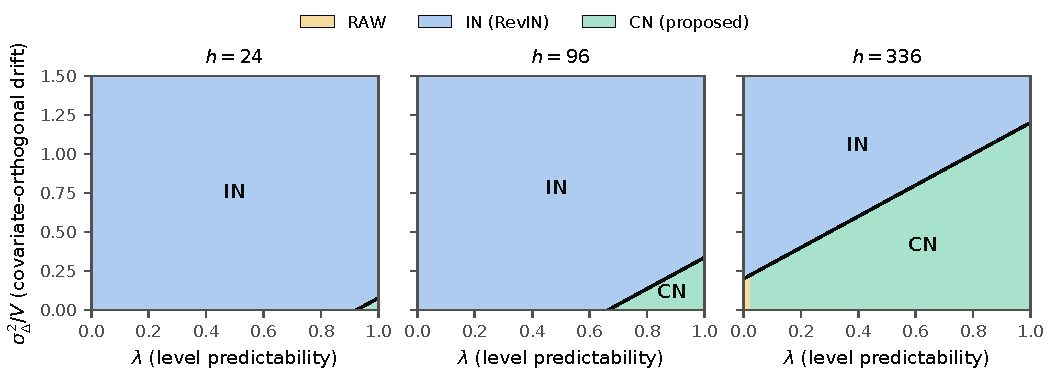
\includegraphics[width=\textwidth]{figures/fig1_dominance.pdf}
  \caption{Dominance map of the three estimators in the $(\lambda,\, \sdel/V)$ plane for $h \in \{24, 96, 336\}$ (left to right). Each region colors the argmin of the closed-form MSEs of \rawm{}, \inm{}, and \cnm{}-est under M1; the curve is the boundary $\lamstar(\sdel)$ of \Cref{eq:lamstar}. Baseline parameters: $V=1$, $w=96$, $\sigma_z=1$, $\sigma_u^2=0.0036$, $\sest=0.02$, $\sx=0$, $\sigma_\varepsilon=0$. On the drift-free axis ($\sdel=0$) the threshold is $\lamstar=0.923$ at $h=24$ and $0.664$ at $h=96$, and $\lamstar<0$ at $h=336$, where \cnm{} dominates for every $\lambda$. Takeaway: as the horizon grows, the \inm{} region retreats upward --- instance normalization survives only under large covariate-orthogonal drift, the regime its original motivation targets.}
  \label{fig:dominance}
\end{figure}

\Cref{fig:dominance} assembles the propositions into a single picture. At short horizons instance normalization is the right default across most of the plane, and covariate-orthogonal drift ($\sdel$) only enlarges its region --- the RevIN regime. As $h$ grows, the within-horizon displacement $\sx + h\sigma_u^2$ accumulates, the boundary $\lamstar(\sdel)$ sweeps down and left, and by $h=336$ conditional normalization dominates at every level of exogenous predictability unless drift is extreme. The remainder of the paper estimates the abscissa of this map from data before training (\Cref{sec:lps}), verifies the predicted boundary on synthetic data whose parameters we control (\Cref{sec:synthetic}), and tests its sign predictions on real series (\Cref{sec:empirical}).

\section{The Level Predictability Score}\label{sec:lps}

The theory of \Cref{sec:theory} locates the \inm/\cnm{} crossover in terms of population quantities that are unobservable before training. This section operationalizes them as a diagnostic that can be computed from raw data and covariates alone, \emph{before} any forecasting model is fit.

\subsection{Definition}

Partition the training series into non-overlapping windows of length $w$ (stride $w$, so that cross-validation blocks are serially decoupled), and let $\bar{y}_i$ and $\bar{x}_i$ denote the target mean and the covariate mean of window $i$. The Level Predictability Score is the pooled out-of-sample $R^2$ of regressing window-level target means on window-level covariate means under expanding chronological cross-validation:
\begin{equation}\label{eq:lpsdef}
\lps \;=\; 1 \;-\; \frac{\sum_{k=1}^{K}\sum_{i\in\mathcal{T}_k}\bigl(\bar{y}_i - \hat{g}_k(\bar{x}_i)\bigr)^2}{\sum_{k=1}^{K}\sum_{i\in\mathcal{T}_k}\bigl(\bar{y}_i - \bar{y}^{\,\mathrm{tr}}_{k}\bigr)^2},
\end{equation}
where $\hat{g}_k$ is a first-stage regressor fit on all windows preceding test block $\mathcal{T}_k$, and the baseline $\bar{y}^{\,\mathrm{tr}}_{k}$ is the \emph{fold-train} mean of $\bar{y}$---never the out-of-sample mean, which would leak test-period level information into the denominator. We use $K=5$ folds with a minimum training fraction of $0.4$. The official instantiation fixes $w=96$ and takes $\hat{g}_k$ to be LightGBM \citep{ke2017lightgbm}, the same first-stage family used by CondNorm, so that $\lps$ measures exactly the information the conditional normalizer will have access to. For multivariate datasets, we average per-channel $\lps$ values, matching the channel-averaged test MSE of the experimental grid. The covariate set is identical to what CondNorm receives: lead-matched archived numerical weather forecasts and calendar harmonics for the exogenous group, calendar harmonics only for the standard benchmarks. A ridge first stage is reported as a sensitivity check but plays no role in the decision rule.

\subsection{Decision rule and threshold}

The diagnostic induces a one-line prescription, which we state in the \emph{negative} form that our evidence supports:
\begin{equation*}
\lps \geq \tau \;\Rightarrow\; \text{do not estimate the level endogenously};
\quad \text{otherwise instance normalization is the safe default},
\end{equation*}
with $\tau = 0.3$ fixed by pre-registration. The positive branch deliberately names no method. What \Cref{sec:empirical} establishes above the threshold is that \emph{several} covariate-conditioned level models---a first-stage regression used alone, a classical dynamic regression, and \cnm---all beat the best instance-normalized arm, and that they do not order among themselves in a stable way; a rule that named one of them would be claiming more than the data supports, and would be wrong on at least one dataset in our own panel. Below the threshold the prescription is directional in the other sense: every covariate-conditioned model we ran loses, so the endogenous default should be retained.

The value $\tau = 0.3$ was fixed in advance from the stylized model of \Cref{sec:theory}: under the parameter mapping of the synthetic study (\Cref{sec:synthetic}), the restoration-rule model M1 places its crossover \Cref{eq:lamstar} at $\lamstar \approx 0.27$--$0.28$ at $h=24$, and because M1 is an \emph{upper bound} on the crossover realized by trained predictors---whose empirical crossings in the synthetic grid occur at $0.01$--$0.03$ (\Cref{sec:synthetic})---adopting $\tau = 0.3$ is conservative toward instance normalization \citep{kim2022revin}. Two qualifications keep this from being read as more than it is. First, $\lps$ is not a consistent estimator of M1's $\lambda$: an out-of-sample $R^2$ nets off first-stage estimation error, so in the notation of \Cref{sec:theory} it behaves like $\lambda - s$ with $s = \sest/V$, and requiring $\lps \geq 0.3$ therefore requires $\lambda \geq 0.3 + s$. This makes the rule \emph{more} conservative toward instance normalization than the nominal threshold suggests, but it also means the anchor is a motivation for the order of magnitude of $\tau$ and not an identity between two coordinates. Second, the threshold is calibrated only in the sense of having been fixed before the data were seen; as \Cref{sec:empirical} reports, our eight datasets are bimodal in $\lps$ with nothing between $0.283$ and $0.744$, so the panel cannot distinguish a sharp crossover at $0.3$ from any cut placed inside that empty interval. Sensitivity of the rule to $\tau$ is quantified in \Cref{tab:tau} and should be read as a robustness check, not as evidence of fine calibration.

The three distinct crossover numbers that appear in this paper, and which of them anchors $\tau$, are set out in \Cref{app:thresholds}.


\subsection{Pre-registration as a falsifiability device}

Because both the diagnostic and the experimental grid are under our control, we bind our hands in advance. Before any grid run was executed, the official $\lps$ value of every dataset and the implied sign of the RevIN$-$CondNorm test-MSE gap were committed to the repository (git commit \texttt{cab17c1}), together with the success criterion (at least $6/8$ sign hits) and the fixed grid design. The pre-registration also flagged, in advance, electricity ($\lps = 0.283$, just below $\tau$) as the cell with the least confident sign prediction. All hits and misses are reported as-is in \Cref{sec:empirical}; the diagnostic is falsifiable, and \Cref{fig:lpsgap} shows the resulting predictions against the realized gaps.

\subsection{A known blind spot}

Absolute $\lps$ has a blind spot we did not resolve: on strongly persistent series (electricity market prices are the canonical example), covariates that are merely \emph{redundant} with the recent history can inflate $\lps$ even though they add nothing beyond what instance normalization already exploits. A natural incremental variant nets off a persistence baseline,
\begin{equation}\label{eq:dlps}
\dlps \;=\; R^2_{\mathrm{oos}}\bigl(\bar{y}_{i+1} \sim \bar{x}_{i+1},\, \bar{y}_i\bigr) \;-\; R^2_{\mathrm{oos}}\bigl(\bar{y}_{i+1} \sim \bar{y}_i\bigr),
\end{equation}
and we report it alongside $\lps$ and the persistence-only $R^2$ in \Cref{tab:tau} for completeness. We make no claim for it: on our eight datasets $\dlps$ never overturns an absolute-$\lps$ verdict, so the panel contains no case that would discriminate between the two, and validating an incremental rule requires the high-persistence, covariate-driven quadrant that our data do not sample. The pre-registered rule is absolute $\lps$ throughout.

\subsection{Why a pre-training diagnostic}

Choosing a normalization by grid search is expensive: our own comparison required 4{,}202 training runs across normalizations, backbones, horizons, and seeds. The $\lps$ computation, by contrast, involves only a handful of window-level first-stage fits---seconds to minutes on a CPU---and requires no forecasting model at all. Beyond cost, a pre-training diagnostic changes the epistemic status of the comparison: rather than selecting a normalization post hoc from test results, the practitioner commits to a choice from data properties alone. This is the move that feature-based forecasting-method selection made for whole methods \citep{talagala2023metalearning, monteromanso2020fforma}, applied here to a single pipeline component, and it answers directly the call of \citet{noise2025signal} for a principled diagnostics-driven strategy to replace the hand-set heuristic whose failure they report.

\section{Synthetic Validation}\label{sec:synthetic}

Before turning to real data, we verify that the crossover characterized in \Cref{sec:theory} materializes under stochastic-gradient training on finite samples, using a data-generating process (DGP) whose exogenous level predictability is known exactly.

\paragraph{Data-generating process}
Covariates follow an AR(1) process, $x_t = 0.9\,x_{t-1} + \epsilon_t$ with $\epsilon_t \sim \mathcal{N}(0,1)$. The series level mixes an exogenously explained component and a covariate-orthogonal random walk,
\[
m_t \;=\; \sqrt{\lambda}\,\beta^\top \tilde{x}_t \;+\; \sqrt{1-\lambda}\,u_t,
\qquad u_t = u_{t-1} + \eta_t,\;\; \eta_t \sim \mathcal{N}(0,\sigma_u^2),
\]
where $\tilde{x}_t$ denotes standardized covariates, so that by construction the population $R^2$ of the level regression equals $\lambda$ (we verify this identity empirically on each generated series). The observed series adds a shape component with daily seasonality, $z_t = A\sin(2\pi t/P) + \rho\,z_{t-1} + \nu_t$ with period $P=24$, giving $y_t = m_t + \sigma_0 z_t$. Thus $\lambda$ is a direct, controllable analogue of the $\lps$ diagnostic of \Cref{sec:lps}.

\paragraph{Sweep design}
We sweep $\lambda \in \{0.0, 0.1, \dots, 1.0\}$ (11 points), horizons $h \in \{24, 96, 336\}$, lookbacks $L \in \{96, 336\}$, ten seeds, and four normalization arms---\rawm{} (global z-score only), RevIN \citep{kim2022revin}, \cnm-oracle (true $m_t$), and \cnm-est (LightGBM first stage \citep{ke2017lightgbm})---for $11 \times 3 \times 2 \times 10 \times 4 = 2{,}640$ runs. Each series has length 20{,}000 with a chronological 6:2:2 train/validation/test split. The backbone is fixed to RLinear \citep{li2023rlinear} in every arm: because the theory of \Cref{sec:theory} is linear-Gaussian, the validation experiment must use a backbone in exactly that function class---a theory--experiment fidelity principle we maintain throughout (capacity is never a confound; only the normalization varies across arms). Nonlinear backbones enter only in the real-data study of \Cref{sec:empirical}.

\paragraph{Gate~1 results}
The experiment was pre-registered as a go/no-go gate with three criteria; all three passed. \Cref{fig:synth} overlays the empirical seed-mean $\mse$ points on the closed-form constrained-OLS theory curves.

\emph{(i) Crossover location.} The empirical IN/CN crossing $\lamstar_{\mathrm{emp}}$ matches the constrained-OLS prediction in all six $(h,L)$ cells, with maximum absolute deviation $0.015$ (criterion: $\pm 0.1$). At $L=96$ the (empirical, theory) pairs are $(0.009, 0.007)$, $(0.011, 0.009)$, and $(0.022, 0.022)$ for $h = 24, 96, 336$; at $L=336$ they are $(0.018, 0.007)$, $(0.023, 0.008)$, and $(0.029, 0.021)$.

\emph{(ii) Horizon monotonicity.} As predicted by \Cref{sec:theory}, the IN--CN gap at fixed $\lambda = 0.8$ widens with $h$: seed-paired increments are $+0.1699 \pm 0.0336$ ($h{=}24 \to 96$) and $+0.0314 \pm 0.0244$ ($h{=}96 \to 336$) at $L=96$, and $+0.1276 \pm 0.0193$ and $+0.0395 \pm 0.0158$ at $L=336$ (95\% confidence intervals).

\emph{(iii) First-stage error.} The degradation of \cnm-est relative to \cnm-oracle is explained by the measured first-stage error $\sest$ inserted into the theory: the median experiment-to-theory degradation ratio is $1.12$, well inside the pre-registered $[0.5, 2.0]$ band.

\paragraph{A discrepancy that sharpens the theory}
The stylized restoration-rule model M1 predicts $\lamstar_{\mathrm{M1}} \approx 0.27$--$0.28$ at these settings, yet the observed crossings lie at $0.009$--$0.029$. The resolution is Proposition~2$'$ (\Cref{sec:theory}): a linear backbone applied to instance- or globally-normalized inputs implicitly performs OLS-style tracking of residual level drift inside the lookback window, so the operative \rawm{} and \cnm{} estimators are strictly stronger than M1's pure restoration rules \citep{toner2024linear}. The constrained-OLS curves---the exact optima within each normalization's function class---capture this and match the experiments; $\lamstar_{\mathrm{M1}}$ is an upper bound, and the $\lamstar_{\mathrm{M1}} - \lamstar_{\mathrm{OLS}}$ gap measures the size of implicit level tracking. The practical implication is notable: when no covariate-orthogonal drift separates train and test ($\sdel = 0$), \cnm{} dominates from very small $\lambda$ onward. Instance normalization's practical niche is therefore drift robustness---precisely the distribution-shift setting that motivated RevIN---rather than level prediction per se, a point we revisit on real data in \Cref{sec:empirical}.

\begin{figure}[t]
  \centering
  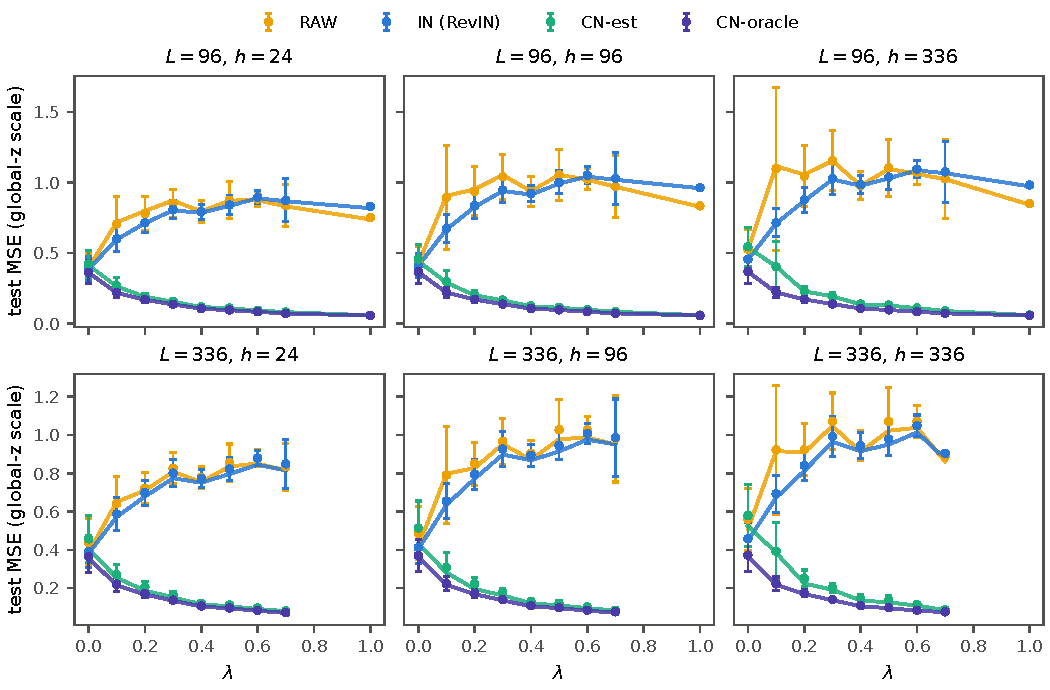
\includegraphics[width=\textwidth]{figures/fig2_synth.pdf}
  \caption{Synthetic validation (Gate~1). Empirical seed-mean test $\mse$ (points, $\pm$1 s.d.\ across ten seeds) overlaid on closed-form constrained-OLS theory curves (lines) for \rawm, RevIN, \cnm-oracle, and \cnm-est as a function of the exogenous level-predictability share $\lambda$, across horizons $h \in \{24, 96, 336\}$ and lookbacks $L \in \{96, 336\}$. Empirical IN/CN crossings match theory within $0.015$; the gap at high $\lambda$ widens with $h$.}
  \label{fig:synth}
\end{figure}

\section{Empirical Study}\label{sec:empirical}

This section reports the pre-registered real-data study. The design tests three falsifiable claims fixed before any grid run (\Cref{sec:lps}): (i) the sign of the RevIN--CondNorm test-error gap on each dataset is predicted by the $\lps$ decision rule with $\tau=0.3$; (ii) the magnitude of the gap increases monotonically with $\lps$; and (iii) on Jeju Wind the gap at $h=48$ exceeds the gap at $h=24$, as \Cref{sec:theory} predicts. Claim (i) constitutes the second pre-registered go/no-go gate (Gate~2); claims (ii) and (iii) are auxiliary predictions excluded from the gate verdict. Three additional blocks probe the mechanisms behind the result; their full tables appear in \Cref{app:ext}.

\subsection{Data}

We use eight datasets in two groups. The \emph{exogenously-driven} group consists of series whose level is substantially determined by observable external drivers. \textbf{Jeju Wind} is aggregate wind-power generation on Jeju Island, Korea (hourly, July 2021--December 2023; 21{,}720 observations), paired with archived short-term numerical weather prediction (NWP) forecasts from the Korea Meteorological Administration. Forecasts are \emph{lead-matched} to the forecast origin: for horizons $h\le 24$ we use the forecast band issued at 23:00 two days prior (lead times 26--49\,h), and for $h\le 48$ the band issued three days prior (lead times 50--73\,h). The correlation between generation and forecast wind speed is $0.742$ for the day-ahead band and $0.704$ for the longer-lead band---decaying with lead time, as physically expected.\footnote{A transparency
note on dataset provenance: Jeju Wind was curated by us during this study
(data collection, NWP lead-matching, and quality screening were interleaved
with method development), so it should be read as a \emph{development}
dataset. GEFCom2014 and the standard long-horizon benchmarks are third-party
datasets frozen before this project began, and play a confirmation-style
role. The distinction does not affect the pre-registration guarantee: the
sign predictions for all eight datasets---including Jeju Wind---were derived
from the $\lps$ rule and committed (commit \texttt{cab17c1}) before any grid
run on any dataset was launched.} A single archive gap (25 June--4 July 2023) is handled by segment-aware windowing: no training or evaluation window spans the gap, and no values are interpolated. The remaining three series---\textbf{GEFCom-Wind}, \textbf{GEFCom-Load}, and \textbf{GEFCom-Solar}---come from GEFCom2014 \citep{hong2016gefcom} with their published explanatory variables (NWP wind components, temperature, and NWP solar variables, respectively).

We emphasize the leakage discipline for weather covariates: all NWP inputs are \emph{archived operational forecasts matched by issue lead}, never reanalysis products. Reanalyses assimilate observations from the forecast target period and would leak future information into the covariate path---a subtle but fatal flaw for any claim about exogenous predictability.

The \emph{standard} group comprises the long-term-forecasting benchmarks ETTh1, ETTh2, Electricity, and Weather. Here the only covariates supplied to any method are deterministic calendar harmonics, so conditional normalization can exploit seasonal structure but has no genuinely exogenous level information. This group is where the distribution-shift motivation of instance normalization \citep{kim2022revin} is expected to hold.

\subsection{Design and protocol}

Block~A, the pre-registered grid, crosses five normalization arms \{Raw, RevIN, SAN, FAN, CondNorm\} \citep{kim2022revin,liu2023san,ye2024fan} with four backbones \{RLinear, PatchTST, SegRNN, LightGBM-DMS\} \citep{li2023rlinear,nie2023patchtst,lin2023segrnn,ke2017lightgbm}, horizons $h\in\{24,96,336\}$ ($\{24,48\}$ for Jeju Wind, constrained by NWP lead coverage), and seeds $\{0,\dots,4\}$; LightGBM runs are deterministic. The combinations LightGBM$\times$SAN and LightGBM$\times$FAN are structurally infeasible (these arms are learned, backpropagated modules) and were declared N/A at pre-registration; the RevIN analogue for LightGBM is per-window z-normalization. Block~A comprises 1{,}794 runs.

Capacity is controlled to isolate the normalization effect: for each (dataset, backbone, $h$), the lookback is tuned over $\{96,192,336,720\}$ on \emph{validation} loss of the RevIN arm at seed~0, then frozen for all five arms. Thus arms within a cell differ in normalization only---never in depth, width, or lookback. Splits are chronological and out-of-time; the global z-score is fit on the training segment only; loaders use \texttt{drop\_last=False} \citep{qiu2024tfb}; training uses fixed seeds and deterministic kernels (full settings in \Cref{app:repro}).

Three extension blocks reuse this discipline. Block~A is deliberately information-asymmetric: only CondNorm consults the covariates (through its first-stage regression), while the four endogenous arms see the target alone. Block~B (\emph{covariate-fair}; 1{,}133 runs) removes this asymmetry, giving \emph{every} arm identical past and future covariates as inputs across five covariate-capable backbones, so that any residual CondNorm advantage cannot be attributed to covariate access. Blocks~C and~D (1{,}275 runs; 4{,}202 in total) run the arms on published state-of-the-art architectures---TimeXer and iTransformer \citep{wang2024timexer,liu2024itransformer}---with (C) and without (D) their official covariate paths; their built-in \texttt{use\_norm} (equivalent to our RevIN arm) is removed so that normalization enters \emph{only} through the five external arms. The backbone-by-backbone correspondence between published defaults and our arms is audited in \Cref{tab:audit} (\Cref{app:design}). Because training budgets differ across blocks (e.g., epoch caps of 12 in~A and 15 in~B), we never compare numbers \emph{across} blocks; each block is internally uniform and self-contained.

\subsection{Statistical testing}

Significance marks use Diebold--Mariano tests \citep{diebold1995comparing} on the per-$(\text{backbone},h)$ seed-mean loss differentials, with a Bartlett-kernel HAC variance (bandwidth $h-1$, capped at $n/4$) and the small-sample correction of \citet{harvey1997testing}. Dataset-level marks in \Cref{tab:main} combine the cell-level $p$-values by Fisher's method ($p<0.05$).\footnote{Fisher's method assumes independent $p$-values, whereas the
per-(backbone,\,$h$) cells within a dataset share the same test period and
are positively dependent, making the combination anti-conservative. As a
robustness check we recombined all cells with two dependence-robust rules:
under the harmonic-mean $p$-value \citep{wilson2019hmp}, valid under
arbitrary dependence, and under Simes's procedure, $31$ of the $32$ stars
in \Cref{tab:main} are unchanged. The single exception is RevIN on ETTh2
(only $3$ of $9$ cells individually significant; Fisher $p=0.026$,
harmonic-mean $p=0.077$, Simes $p=0.130$), which should be read as
indicative; the qualitative conclusion for ETTh2 (instance normalization
dominates conditional normalization by a wide margin) does not rest on
this mark.} Complementing pairwise tests, we compute the Model Confidence Set \citep{hansen2011mcs} over the five arms within each (dataset, $h$) cell at $\alpha=0.10$, using the $T_{\max}$ statistic and the stationary bootstrap \citep{politis1994stationary}.

\subsection{Pre-registered results}

\begin{table}[t]
\centering
\caption{Main results by dataset. Columns are grouped into \emph{benchmarks} (deterministic, no learned normalization), \emph{endogenous} level handling (the instance-normalization family, plus global $z$-scoring which handles the level with a single train-fitted constant), and \emph{exogenous} level handling. Panel~(a): test MSE on the train-fitted global $z$-score scale, averaged over backbones, horizons, and seeds (Block~A). Panel~(b): the same forecasts in MASE, i.e.\ test MAE divided by the in-sample seasonal-naive MAE of the same series on the same scale \citep{hyndman2006another}, so values are comparable across datasets and $>1$ means worse than a one-step seasonal-naive benchmark fitted in-sample. \textbf{Bold}: row minimum over all nine columns. $^{*}$: significantly worse than the best \emph{normalization} arm ($p<0.05$; DM test with Harvey correction on per-$(\text{backbone},h)$ seed-mean loss differentials, Fisher-combined across cells); the DM machinery is defined within Block~A, so the four benchmark columns carry no marks. Benchmarks are run on the identical chronological splits, window-admissibility rules and $z$-scale as Block~A at the fixed lookback $L=336$ (\Cref{app:ext}); they are deterministic and therefore have no seed variation.}
\label{tab:main}
\small
\setlength{\tabcolsep}{3.2pt}
\begin{tabular}{lcccccccccc}
\toprule
& \multicolumn{4}{c}{Benchmarks} & \multicolumn{4}{c}{Endogenous level} & Exogenous \\
\cmidrule(lr){2-5}\cmidrule(lr){6-9}\cmidrule(lr){10-10}
Dataset & S.\,naive & Clim. & DynReg & FirstStg & Raw & RevIN & SAN & FAN & CondNorm \\
\midrule
\multicolumn{10}{l}{\emph{(a) Test MSE}} \\[2pt]
\multicolumn{10}{l}{\emph{Exogenously-driven group}} \\
Jeju Wind     & $1.6265$ & $1.0320$ & $\mathbf{0.2850}$ & $0.2938$ & $0.6887^{*}$ & $0.6969^{*}$ & $0.7030^{*}$ & $0.7724^{*}$ & $0.2933$ \\
GEFCom-Wind   & $1.9878$ & $1.2312$ & $0.1710$ & $\mathbf{0.1564}$ & $1.1153^{*}$ & $1.0039^{*}$ & $0.9755^{*}$ & $1.1875^{*}$ & $0.1629$ \\
GEFCom-Load   & $0.6860$ & $1.1900$ & $0.3714$ & $0.1365$ & $0.3592^{*}$ & $0.3432^{*}$ & $0.3330^{*}$ & $0.3678^{*}$ & $\mathbf{0.1066}$ \\
GEFCom-Solar  & $0.3329$ & $0.2029$ & $0.1414$ & $\mathbf{0.0565}$ & $0.1828^{*}$ & $0.1844^{*}$ & $0.2116^{*}$ & $0.1833^{*}$ & $0.0580$ \\
\midrule
\multicolumn{10}{l}{\emph{Standard LTSF group}} \\
ETTh1         & $0.6695$ & $0.8826$ & $0.4792$ & $1.4033$ & $0.3962^{*}$ & $\mathbf{0.3771}$ & $0.3910^{*}$ & $0.4114^{*}$ & $2.2016^{*}$ \\
ETTh2         & $0.5769$ & $3.1284$ & $0.8921$ & $3.3670$ & $0.3868^{*}$ & $0.2900^{*}$ & $\mathbf{0.2869}$ & $0.3253^{*}$ & $6.6044^{*}$ \\
Electricity   & $0.2174$ & $0.3894$ & $0.1986$ & $0.3224$ & $0.1500^{*}$ & $0.1458^{*}$ & $0.1443^{*}$ & $\mathbf{0.1375}$ & $0.1726^{*}$ \\
Weather       & $0.3383$ & $0.6876$ & $0.1808$ & $0.6483$ & $0.1815^{*}$ & $0.1719^{*}$ & $\mathbf{0.1666}$ & $0.1747^{*}$ & $0.7274^{*}$ \\
\midrule
\multicolumn{10}{l}{\emph{(b) MASE}} \\[2pt]
\multicolumn{10}{l}{\emph{Exogenously-driven group}} \\
Jeju Wind     & $1.121$ & $1.030$ & $\mathbf{0.462}$ & $0.477$ & $0.776$ & $0.741$ & $0.761$ & $0.803$ & $0.478$ \\
GEFCom-Wind   & $1.225$ & $0.985$ & $0.350$ & $\mathbf{0.335}$ & $0.921$ & $0.885$ & $0.881$ & $0.950$ & $0.345$ \\
GEFCom-Load   & $1.613$ & $2.310$ & $1.186$ & $0.687$ & $1.155$ & $1.123$ & $1.113$ & $1.166$ & $\mathbf{0.564}$ \\
GEFCom-Solar  & $1.288$ & $1.197$ & $1.253$ & $\mathbf{0.554}$ & $1.220$ & $1.239$ & $1.369$ & $1.212$ & $0.587$ \\
\midrule
\multicolumn{10}{l}{\emph{Standard LTSF group}} \\
ETTh1         & $1.219$ & $1.691$ & $1.114$ & $2.064$ & $1.006$ & $\mathbf{0.950}$ & $0.966$ & $1.024$ & $2.549$ \\
ETTh2         & $1.535$ & $4.254$ & $1.963$ & $4.362$ & $1.288$ & $\mathbf{1.090}$ & $1.092$ & $1.192$ & $5.691$ \\
Electricity   & $1.047$ & $1.605$ & $1.089$ & $1.423$ & $0.947$ & $0.926$ & $0.930$ & $\mathbf{0.881}$ & $0.995$ \\
Weather       & $0.754$ & $1.503$ & $0.633$ & $1.237$ & $0.602$ & $\mathbf{0.532}$ & $0.537$ & $0.566$ & $1.300$ \\
\bottomrule
\end{tabular}
\end{table}

\Cref{tab:main} is the paper's central result, and it is a double dissociation between two \emph{strategies} for handling the level, not a ranking of methods. Read the three covariate-conditioned columns---the first-stage regression used alone, the classical dynamic regression, and \cnm---against the best instance-normalized arm in each row. On the exogenously-driven group they win $11$ of the $12$ comparisons; on the standard group they win $0$ of $12$. Under MASE the counts are $10$ of $12$ and $0$ of $12$. Both exceptions are the same method for the same reason: the ridge \emph{DynReg} loses on GEFCom-Load, whose temperature--load response is strongly nonlinear---the identical failure that costs a ridge first stage two hits in the $\lps$ sensitivity check of \Cref{tab:tau}---and, under MASE only, on GEFCom-Solar. No covariate-conditioned model wins on any standard dataset under either measure.

Three further readings matter. First, the effect is not an artifact of a dimensionless scale: panel~(b) puts every number against the same series' own in-sample seasonal-naive error, and the ordering is unchanged. Second, the benchmark columns discipline the interpretation in both directions---on GEFCom-Load and GEFCom-Solar \emph{every} endogenous arm is worse than an in-sample seasonal-naive benchmark (MASE $1.11$--$1.37$), which is the operationally meaningful statement of what the boundary costs, while on the standard group the endogenous arms sit at MASE $0.53$--$1.09$ and the covariate-conditioned ones at $0.99$--$5.69$. Third, the failure of \cnm{} off its region is severe and we do not soften it: on ETTh2 it reaches MSE $6.6044$ against $0.2869$ for the best arm, because calendar harmonics carry essentially no level information and the first-stage regression injects its own error into the restored level. \Cref{sec:discussion} reports what a shrinkage safeguard does and does not repair.

\paragraph{Gate~2: sign predictions} All eight pre-registered sign predictions were confirmed (criterion: at least 6/8). The realized dataset-mean gaps, $\mse(\text{RevIN})-\mse(\text{CondNorm})$, are: Jeju Wind $+0.4037$, GEFCom-Wind $+0.8410$, GEFCom-Load $+0.2366$, GEFCom-Solar $+0.1264$ (all predicted positive), and ETTh1 $-1.8244$, ETTh2 $-6.3145$, Electricity $-0.0268$, Weather $-0.5555$ (all predicted negative). These predictions, the official $\lps$ specification, and $\tau=0.3$ were committed to version control (commit \texttt{cab17c1}) before any grid run was launched.

What this record does and does not show is worth stating precisely, because the natural summary statistic is misleading here. A binomial reference treating each sign as a coin flip would give $2^{-8}\approx 0.004$, but the eight datasets are not eight independent draws: they fall into two internally correlated regimes, and a reader who grants only that the two \emph{regimes} were called correctly is looking at $p = 0.25$. We therefore do not rest any claim on the aggregate hit rate. The informative content is per-dataset and is robust in the ways that can be checked without new runs: the same eight signs are obtained under MAE and under MASE (\Cref{tab:main}b), so the record is not an artifact of squared error on a dimensionless scale; the margins are large relative to seed dispersion on seven of the eight datasets, Electricity being the exception by construction; and the per-dataset magnitudes in \Cref{tab:main} do not depend on treating the datasets as exchangeable. What the record establishes is that a quantity computable before training assigned each of our eight series to the correct side of the boundary; what it cannot establish, with eight series in two clusters, is a calibrated probability that it will do so on the next one.

\paragraph{Model Confidence Sets} At $\alpha=0.10$, the surviving set in \emph{all eleven} exogenous (dataset, $h$) cells is $\{\text{CondNorm}\}$ alone. On the standard cells the survivors are $\{\text{RevIN}\}$ in all three ETTh1 cells, $\{\text{RevIN},\text{SAN}\}$ in all three ETTh2 cells, $\{\text{FAN}\}$ in all three Electricity cells, and $\{\text{SAN}\}$ in all three Weather cells. Across all 23 cells, survival counts are: Raw 0, RevIN 6, SAN 6, FAN 3, CondNorm 11. One property of this output should temper how it is read: the procedure returns a \emph{singleton} in 20 of the 23 cells. A confidence set that almost always contains exactly one element is reporting an ordering rather than quantifying uncertainty about it, which is what one expects when the bootstrap resamples a single realized test path and the arms have been averaged over backbones and seeds beforehand. We therefore treat the model confidence sets as a compact summary of the within-cell ranking, consistent with the pairwise tests, and not as an independent uncertainty statement; the limitation is the single evaluation origin discussed in \Cref{sec:discussion}, which no post-processing of these runs can repair.

\paragraph{The near-boundary case} Electricity sits closest to the threshold ($\lps=0.283<\tau=0.3$) and was flagged in the pre-registration as the lowest-confidence prediction. It behaved accordingly: its realized gap is the smallest in magnitude ($-0.0268$), roughly five times closer to zero than any other dataset, so the boundary is where the two regimes genuinely meet rather than an artifact of dataset selection. We are careful, though, not to overstate how densely the boundary is sampled. The $\lps$ values are strongly bimodal---$0.74$--$0.89$ for the four energy series and $-0.72$--$0.28$ for the four standard benchmarks---with no dataset in between; the wide all-correct plateau of \Cref{tab:tau} ($\tau\in[0.30,0.70]$) therefore falls entirely in this empty inter-cluster gap and reflects the separation between the two regimes as much as any fine calibration of $\tau$. Electricity is the only dataset that lands near the threshold at all, so the rule is genuinely stress-tested at its boundary in effectively a single case ($n=1$). Establishing that the crossover is \emph{sharp} there---rather than that two well-separated clusters are merely distinguishable---will require datasets of intermediate predictability, which we flag as a target for confirmatory replication.

\subsection{Mechanism: the layer, not the information}\label{sec:parity}

\Cref{tab:main} is deliberately information-asymmetric: only \cnm{} consults the covariates, through its first-stage regression, while the four endogenous arms see the target alone. Taken by itself the table is therefore consistent with the objection that this is ``just feature engineering''---a model that sees tomorrow's weather forecast beats models that do not. The information-parity block (Block~B; 1{,}133 runs) removes the asymmetry by supplying \emph{every} arm with the identical past and future covariates as backbone inputs, across five covariate-capable backbones, on the four exogenously-driven datasets. This is the comparison that carries the paper's mechanism claim, so we report it with uncertainty rather than as point estimates.

The operative quantity is the \emph{isolated cost of the normalization layer under equal information}: the paired difference $\mse(\text{RevIN}+\text{cov}) - \mse(\rawm+\text{cov})$, in which the two arms receive the same inputs, the same backbone, the same capacity and the same budget, and differ only in whether the window statistics are removed and mechanically restored. It is positive on every backbone:

\begin{center}
\small
\begin{tabular}{lccc}
\toprule
Backbone & $\mse(\text{RevIN}+\text{cov}) - \mse(\rawm+\text{cov})$ & 95\% CI & cells $>0$ \\
\midrule
LGBM-Cov      & $+0.0191$ & $[+0.0116,\, +0.0269]$ & 11/11 \\
Linear mixer  & $+0.0205$ & $[+0.0056,\, +0.0368]$ & 8/11 \\
MLP mixer     & $+0.0238$ & $[+0.0119,\, +0.0390]$ & 10/11 \\
SegRNN-Cov    & $+0.0112$ & $[+0.0058,\, +0.0172]$ & 10/11 \\
PatchTST-Cov  & $+0.0038$ & $[-0.0091,\, +0.0167]$ & 7/11 \\
\bottomrule
\end{tabular}
\end{center}

\noindent Intervals are cluster bootstraps over the 11 seed-averaged (dataset, horizon) cells, resampling cells rather than origins so that the serial dependence within a test path is not treated as replication. Four of the five differences exclude zero; \textbf{PatchTST-Cov does not}, and we state that as a null rather than absorbing it into a claim about ``every backbone''---its minimal covariate adapter exposes less level information to the backbone than the other four, so it is the arm in which the layer has least to destroy. The magnitudes deserve equal candour: these are differences of $0.004$ to $0.024$ MSE, one to two orders of magnitude below the $+0.841$ headline gap of \Cref{tab:main}. That contrast is the honest shape of the result. The large number measures what covariate access is worth; the small number measures what the normalization layer costs once access is equalized, and only the small number is attributable to the layer.

Two further observations sharpen the mechanism. First, the \rawm$-$\cnm{} gap shrinks as backbone flexibility grows ($+0.127$ for the linear mixer, $+0.052$ for the MLP mixer, $-0.009$ for LightGBM-Cov, i.e.\ \rawm{} slightly ahead), while the RevIN$-$\rawm{} difference above persists at every capacity. A flexible model given raw inputs can learn the covariate-to-level map for itself, which is why \cnm{} loses its advantage there; no model can recover a level its normalizer has already subtracted, which is why the RevIN penalty does not vanish. This is the reparameterization argument of \citet{toner2024linear} applied to a constrained rather than an unconstrained class. We flag the capacity ordering as an exploratory post-hoc observation confined to the mixer ladder: PatchTST-Cov ($+0.142$) sits outside it and SegRNN-Cov is $-0.004$. Second, this is the same dissociation that \Cref{tab:main} shows at the level of strategies, obtained by a different route---there by comparing methods that condition the level on covariates against methods that do not, here by holding the covariates fixed and toggling only the layer.

\subsection{What \texorpdfstring{$\lps$}{LPS} orders, and what it does not}

\begin{figure}[t]
\centering
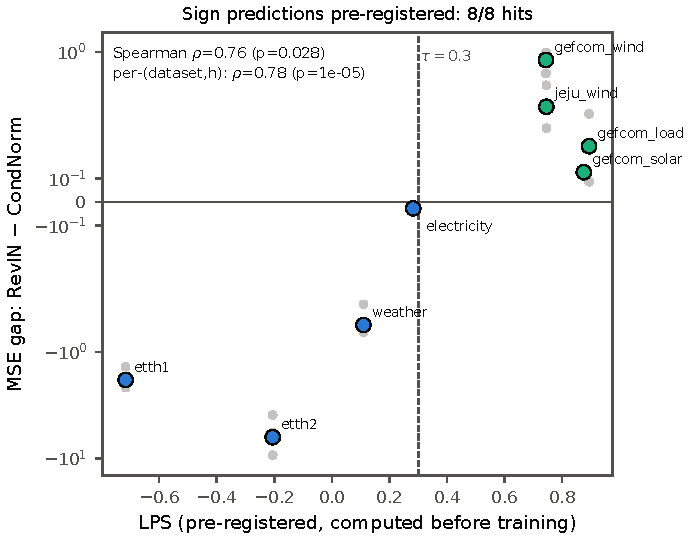
\includegraphics[width=.75\linewidth]{figures/fig3_lps_gap.pdf}
\caption{Realized RevIN$-$CondNorm test-MSE gap versus pre-registered $\lps$, one point per (dataset,\,$h$) cell, coloured by regime. The vertical line marks $\tau=0.3$. The pooled rank association ($\rho=0.783$, $n=23$) is a \emph{between}-regime effect: within the exogenously-driven regime the association reverses ($\rho=-0.750$, $n=11$), so the figure should be read as a separation of two clusters, not as a dose--response curve.}
\label{fig:lpsgap}
\end{figure}

Beyond sign accuracy, the pre-registration recorded an auxiliary prediction (excluded from the gate) that the gap \emph{magnitude} increases with $\lps$. \textbf{We report this prediction as not supported.} Pooled over all 23 (dataset, $h$) cells the rank association is positive and large, $\rho=0.783$; but decomposing it by regime shows that it is entirely a between-cluster effect. Within the exogenously-driven regime the association \emph{reverses}: $\rho=-0.750$ on its 11 cells, and the two datasets with the highest $\lps$ (GEFCom-Load $0.894$ and GEFCom-Solar $0.875$) have the two \emph{smallest} dataset-mean gaps ($+0.237$ and $+0.126$), while the two lowest-$\lps$ exogenous datasets have the largest ($+0.841$ and $+0.404$). Within the standard regime the association is positive ($\rho=+0.777$ on 12 cells). A pooled coefficient computed across two well-separated clusters measures the separation, not an ordering inside either one, and the nominal $p$-values that accompany it are not valid in any case: the 23 cells are nested within eight datasets, and an exact permutation test that respects the cluster structure gives $p=0.023$ rather than the nominal $9.9\times10^{-6}$.

The honest conclusion is narrower than the pre-registered prediction and we adopt it throughout: $\lps$ is demonstrated here as a \emph{regime classifier}---it places a series on the correct side of the boundary---and not as a calibrated measure of how much is at stake once a series is on the exogenous side. Establishing the latter requires series with genuinely graded level predictability rather than two clusters, which our panel does not contain; we return to this in \Cref{sec:discussion}.

\begin{table}[t]
\centering
\caption{The $\lps$ decision rule. Panel (a): number of correct sign predictions (out of 8) as the threshold $\tau$ varies; the pre-registered $\tau=0.3$ lies in the widest all-correct plateau. Panel (b): per-dataset diagnostics; $\dlps$ is the incremental covariate $R^2$ beyond persistence (\Cref{eq:dlps}) and $R^2_{\mathrm{pers}}$ the persistence-only $R^2$; verdict CN if $\lps\ge\tau$, IN otherwise; realized gap is dataset-mean $\mse(\text{RevIN})-\mse(\text{CondNorm})$.}
\label{tab:tau}
\small
\begin{tabular}{lccccc}
\multicolumn{6}{l}{(a) Threshold sensitivity} \\
\toprule
$\tau$ range & $[0.00,0.10]$ & $[0.15,0.25]$ & $[0.30,0.70]$ & $[0.75,0.85]$ & $0.90$ \\
\midrule
Sign hits / 8 & 6 & 7 & \textbf{8} & 6 & 4 \\
\bottomrule
\end{tabular}

\vspace{1ex}

\begin{tabular}{lccccc}
\multicolumn{6}{l}{(b) Per-dataset verdicts ($\tau=0.3$)} \\
\toprule
Dataset & $\lps$ & $\dlps$ & $R^2_{\mathrm{pers}}$ & Realized gap & Verdict \\
\midrule
Jeju Wind    & $0.745$  & $0.742$  & $0.00$  & $+0.404$ & CN \\
GEFCom-Wind  & $0.744$  & $0.773$  & $-0.01$ & $+0.841$ & CN \\
GEFCom-Load  & $0.894$  & $0.335$  & $0.56$  & $+0.237$ & CN \\
GEFCom-Solar & $0.875$  & $0.556$  & $0.32$  & $+0.126$ & CN \\
ETTh1        & $-0.717$ & $-0.142$ & $0.47$  & $-1.824$ & IN \\
ETTh2        & $-0.205$ & $-0.028$ & $0.45$  & $-6.314$ & IN \\
Electricity  & $0.283$  & $0.031$  & $0.64$  & $-0.027$ & IN \\
Weather      & $0.110$  & $0.558$  & $-0.12$ & $-0.556$ & IN \\
\bottomrule
\end{tabular}
\end{table}

\Cref{tab:tau} probes the robustness of the decision rule itself. The 8/8 hit rate is maintained for every $\tau\in[0.30,0.70]$---a wide plateau containing the pre-registered value---and degrades only outside it (6/8 on $[0.00,0.10]$ and $[0.75,0.85]$, 7/8 on $[0.15,0.25]$, 4/8 at $0.90$). The conclusion does not hinge on a lucky threshold. As the pre-registered sensitivity check, replacing the LightGBM first stage with ridge regression scores 6/8 at the same $\tau$: it misses GEFCom-Load, whose temperature--load response is strongly nonlinear, and Weather---which is precisely why the official rule fixes a nonlinear first stage from the same family CondNorm uses. Panel~(b) lists each dataset's $\lps$, the incremental $\dlps$ of \Cref{eq:dlps} with the persistence-only $R^2_{\mathrm{pers}}$, the realized gap, and the rule verdict; all eight verdicts match the realized sign. The $\dlps$ column adds three readings. First, on the exogenous group the level signal is genuinely exogenous: for the two wind datasets persistence alone explains essentially nothing ($R^2_{\mathrm{pers}}\approx 0$), and even where persistence is strong, covariates add a large increment ($+0.34$ for load, $+0.56$ for solar). Second, the two cells the pre-registration was least sure about are cleanly diagnosed: ETTh2's calendar covariates add nothing beyond persistence ($\dlps=-0.028$), and Electricity---flagged in advance as the least confident sign prediction---combines the strongest persistence in the panel ($0.64$) with an almost-zero increment ($\dlps=0.031$), matching its near-zero realized gap. Third, $\dlps$ is a \emph{secondary} diagnostic for the high-persistence regime, not a replacement rule: Weather has no persistent level ($R^2_{\mathrm{pers}}=-0.12$), so its moderate $\dlps$ (driven by seasonal harmonics) carries no override, and the pre-registered absolute-$\lps$ verdict stands.

We also make the ordering of evidence explicit, since a threshold that
performs well on a grid invites the suspicion that it was tuned on that
grid. It was not: $\tau = 0.3$ was fixed from theory---the stylized upper
bound $\lamstar_{\mathrm{M1}} \approx 0.27$--$0.28$ of
\Cref{sec:theory}---and committed together with all eight sign predictions
(commit \texttt{cab17c1}) before any grid run was launched. The
$[0.30, 0.70]$ plateau of \Cref{tab:tau} is therefore a \emph{post-hoc}
robustness finding, reported as such, not part of the pre-registered
procedure. The sensitivity table also shows that the conclusion survives
moderate misplacement of the threshold: even $\tau = 0.25$, below the
plateau, yields $7/8$ sign hits---still clearing the pre-registered
$\ge 6/8$ bar---and the rule degrades gradually ($6/8$ on $[0.00,0.10]$
and $[0.75,0.85]$) rather than collapsing outside the plateau.

\subsection{Variance attribution}

\begin{table}[t]
\centering
\caption{Variance attribution of log test MSE across Block~A factors (percent of total).}
\label{tab:attribution}
\small
\begin{tabular}{lr}
\toprule
Factor & Share (\%) \\
\midrule
Normalization (main)            & 0.73 \\
Backbone (main)                 & 0.13 \\
Dataset (main)                  & 42.45 \\
Horizon (main)                  & 5.65 \\
Normalization $\times$ dataset  & 47.12 \\
Normalization $\times$ backbone & 0.31 \\
Backbone $\times$ dataset       & 0.44 \\
\bottomrule
\end{tabular}
\end{table}

\begin{figure}[t]
\centering
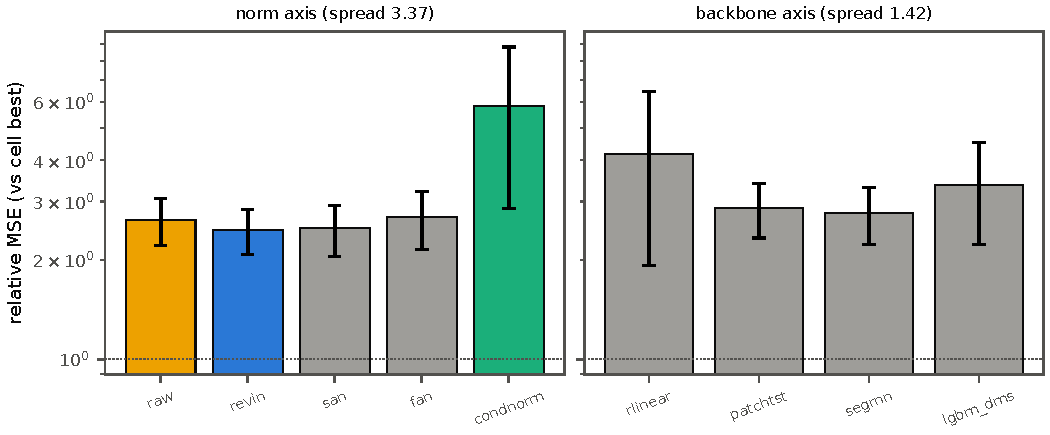
\includegraphics[width=.7\linewidth]{figures/fig4_factors.pdf}
\caption{Factor-level view of the variance attribution in \Cref{tab:attribution}: the normalization effect on error is almost entirely carried by its interaction with the dataset.}
\label{fig:factors}
\end{figure}

\Cref{tab:attribution} decomposes the variance of log test MSE over Block~A. Normalization-related terms account for $48.2\%$ of the variance, backbone-related terms for $0.6\%$. Strikingly, the normalization \emph{main} effect is tiny ($0.73\%$) while the normalization$\times$dataset interaction dominates ($47.12\%$): averaged over datasets, no normalization is better, because the \emph{sign} of the effect flips across datasets. That interaction is not a nuisance term---it \emph{is} the applicability boundary this paper characterizes (\Cref{fig:factors}). By contrast, which backbone sits under the normalization barely matters.

One decomposition of this decomposition is essential to reading it correctly, and we report it rather than leaving it to be found: the $47.12\%$ is carried by the single exogenous arm. Restricting the same computation to the four \emph{endogenous} arms \{\rawm, RevIN, SAN, FAN\}, the normalization$\times$dataset interaction falls to $0.43\%$ and all normalization-related terms total $0.73\%$, against $0.43\%$ for backbone-related terms. A reader could take this as deflating the headline; we take it as sharpening it. Within the endogenous family the choice of normalization is close to immaterial and no more consequential than the choice of backbone---which is consistent with the leaderboard literature, where these arms trade places across benchmarks without a stable winner. The variance that the normalization factor explains appears only when the family is widened to include an arm whose level statistics come from outside the target series. The boundary this paper characterizes therefore runs between endogenous and exogenous level handling, not between RevIN and its endogenous successors, and the attribution is best read as evidence for \emph{where} the boundary lies rather than as a claim that normalization is the dominant design axis in general.

\subsection{Horizon interaction}

\begin{figure}[t]
\centering
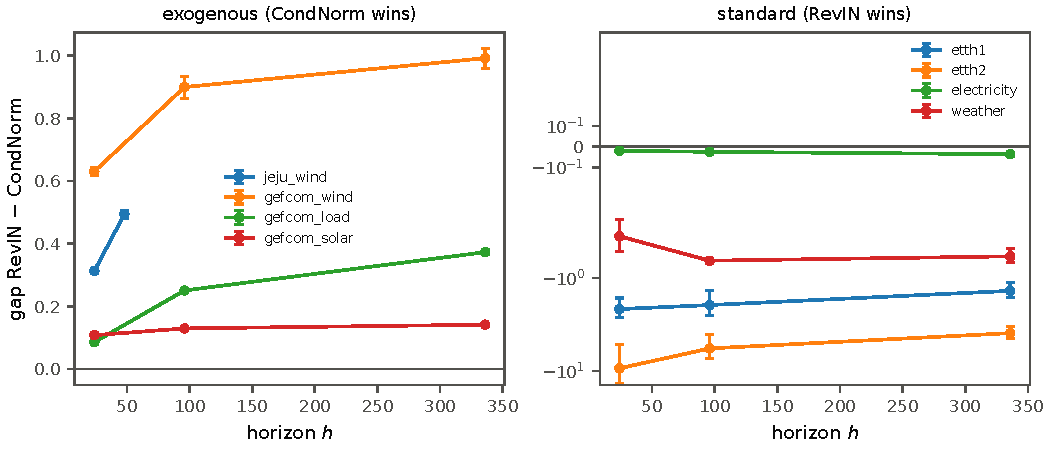
\includegraphics[width=.85\linewidth]{figures/fig5_horizon.pdf}
\caption{RevIN$-$CondNorm gap by horizon on the exogenously-driven group. The gap grows monotonically with $h$ on all four datasets, as predicted by \Cref{eq:prop3}.}
\label{fig:horizon}
\end{figure}

\Cref{sec:theory} predicts that the penalty of the frozen-statistics restoration rule grows with the horizon, since $\sx$ accumulates while the window statistics do not (\Cref{eq:prop3}). \Cref{fig:horizon} shows exactly this on real data: the RevIN$-$CondNorm gap increases monotonically in $h$ on all four exogenously-driven datasets. In particular, the Jeju Wind gap at $h=48$ exceeds that at $h=24$, an auxiliary prediction fixed in the pre-registration document. The horizon interaction confirmed on the synthetic grid (\Cref{sec:synthetic}) thus transfers to operational data.

\subsection{Robustness blocks}

\paragraph{Information parity (Block B)} Reported as the mechanism result in \Cref{sec:parity}; for completeness, within that block \cnm{} attains the lowest mean MSE for three of the five backbones (the linear mixer, the MLP mixer, and PatchTST-Cov) and is within $0.01$ of the best arm (\rawm$+$covariates) for LightGBM-Cov and SegRNN-Cov, so it is an adequate instrument but not the best method even here. By the Harvey-corrected DM test it is significantly better than RevIN in 11/11 exogenous cells for PatchTST-Cov, 10/11 for the linear and MLP mixers, 3/11 for LightGBM-Cov, and 2/11 for SegRNN-Cov. Full tables in \Cref{tab:covfair} (\Cref{app:ext}).

\paragraph{Published covariate architectures (Block C) and endogenous SOTA (Block D)} The pattern is not an artifact of our minimal covariate adapters. On the published covariate paths of TimeXer and iTransformer \citep{wang2024timexer,liu2024itransformer}---with built-in normalization removed and our five arms injected externally---the mean RevIN$-$CondNorm gap is $+0.4122$ for TimeXer-MS (55 pairs) and $+0.4282$ for iTransformer-MS, and CondNorm is best on all four exogenous datasets for both architectures (\Cref{tab:sota}, \Cref{app:ext}). Block~D, running the same architectures in their endogenous multivariate mode, reproduces the Block~A pattern qualitatively: CondNorm wins the exogenous group and loses the standard group.

\paragraph{Adaptive normalization and benchmark sanity} Two remaining objections fall to results already in \Cref{tab:main}. Against ``adaptive normalization already solves this'': SAN and FAN \citep{liu2023san,ye2024fan}, which learn non-stationary statistics rather than conditioning on covariates, lose to CondNorm on the \emph{entire} exogenous group---adapting the statistics endogenously is not a substitute for exogenous level information. Against ``the evaluation is biased toward energy data'': on the standard group our arms reproduce the literature's ranking and error levels (e.g., RevIN-family bests ETTh1 at $0.3771$), consistent with published results for these backbones \citep{li2023rlinear,qiu2024tfb}, and our conclusion there is precisely that instance normalization wins---the boundary, not either side of it, is the finding \citep{brigato2026champions}.

\section{Discussion}\label{sec:discussion}

\subsection{The applicability boundary as the object of study}

The central empirical fact of this paper is not that any single normalization wins, but that the \emph{sign} of the instance-normalization effect flips across datasets in a way that is predictable before training. The variance attribution of \Cref{sec:empirical} (\Cref{tab:attribution}) makes this precise: the norm main effect explains only $0.73\%$ of log-MSE variance, while the norm$\times$dataset interaction explains $47.12\%$---normalization-related terms total $48.2\%$, against $0.6\%$ for all backbone-related terms. A small main effect with a large interaction is exactly the signature of an applicability boundary: averaged over datasets the normalization choice looks unimportant, yet within any given dataset it is close to decisive. This observation also explains why leaderboard-style comparisons on a fixed benchmark suite can be simultaneously reproducible and uninformative about deployment: whether instance normalization helps depends on a property of the data-generating process, not of the model, echoing recent warnings about benchmark monoculture in long-term forecasting \citep{brigato2026champions,position2025benchmark}.

For practitioners the boundary is actionable because it is cheap to locate. Our recommendation is procedural: before committing to a normalization scheme, compute $\lps$ from the covariates already at hand (\Cref{sec:lps}); if $\lps > \tau$ with $\tau = 0.3$, prefer conditional normalization, otherwise retain instance normalization. The rule is not fragile in the threshold: the pre-registered $8/8$ sign predictions are maintained for every $\tau \in [0.30, 0.70]$ (\Cref{tab:tau}), so the decision requires only that the series fall on the correct side of a wide band, not a finely tuned cut point. We emphasize that this is a characterization, not a rebuttal, of RevIN \citep{kim2022revin}: on the standard benchmarks, where the level is not exogenously predictable, the distribution-shift motivation holds and instance-normalization variants remain in every model confidence set.

\subsection{Capacity and the marginal utility of conditional normalization}

The covariate-fair experiments of Block B refine \emph{what} conditional normalization contributes. When all arms receive identical past and future covariates, the \rawm-versus-\cnm{} gap shrinks monotonically along the mixer capacity ladder: $+0.127$ for the linear mixer, $+0.052$ for the MLP mixer, and $-0.009$ (Raw slightly ahead) for gradient-boosted trees. This is exactly the pattern implied by the reparameterization argument of \citet{toner2024linear}: for a sufficiently unconstrained function class with access to the same information, an input-side normalization is absorbable into the hypothesis space, so its marginal value must vanish. We flag this capacity narrative as an exploratory post-hoc observation, not a pre-registered result, and it is confined to the mixer ladder: PatchTST-Cov ($+0.142$) sits outside the ordering---its minimal covariate adapter exposes less level information to the backbone---and SegRNN-Cov is $-0.004$. The \inm-versus-\cnm{} gap, by contrast, \emph{persists at every capacity}---indeed, RevIN-plus-covariates is worse than \rawm-plus-covariates for every Block~B backbone. This is not a capacity phenomenon but a function-class constraint (\Cref{sec:theory}, Proposition~1): instance normalization projects out the window level before the backbone sees the data, and no amount of downstream flexibility can recover information that the covariates carry about a component that has been subtracted and will be mechanically restored. The refined claim is therefore: the value of \cnm{} is (i) repairing constrained deep pipelines whose built-in normalization discards a predictable level, and (ii) providing a modular route for injecting exogenous level information without redesigning the backbone---not a claim that covariate information is unusable any other way.

\subsection{The cost of conditional normalization when it fails}

The boundary cuts both ways, and the failure mode is not mild. On ETTh1, CondNorm reaches mean MSE $2.2016$ against $0.3771$ for RevIN; on ETTh2, $6.6044$ against $0.2869$ for the best arm (\Cref{tab:main}). The mechanism is first-stage error propagation: when $\lambda \approx 0$ the covariates carry no level signal, the first-stage regression fits noise, and the denormalization step injects that noise directly into the forecast---the $\sest$ term of the \cnm{}-est closed-form risk (\Cref{eq:app-msecn}), which is paid in full precisely when there is no offsetting reduction in the level variance to be explained. The catastrophic magnitudes on the standard benchmarks are thus not an implementation artifact but the predicted behaviour of the estimator outside its applicability region, and they are the reason the decision rule exists at all. A natural safeguard is shrinkage: if the first-stage validation $R^2$ is non-positive, shrink the estimated level $\hat m$ toward the global training mean, which recovers the \rawm{} estimator in the limit. We propose this as an extension and deliberately do \emph{not} apply it post hoc to any number reported in this paper, since doing so would blunt exactly the failure the theory predicts and the pre-registration was designed to test.

\subsection{The persistence blind spot and \texorpdfstring{$\dlps$}{Delta-LPS}}

The absolute $\lps$ has a known blind spot: strongly persistent, covariate-driven series---system marginal prices are the canonical example---can score a high $\lps$ even when the covariates add little beyond what the recent history already implies, because covariates and lagged levels are themselves collinear. The incremental diagnostic $\dlps$ (\Cref{sec:lps}) is the refinement: it measures the covariate contribution \emph{over} a persistence baseline. Our theoretical expectation for this quadrant is regime-dependent: in calm regimes instance normalization should remain adequate (persistence carries the level), while conditional normalization should earn its keep at regime shifts, where the covariates lead and the window statistics lag. We leave this as a targeted stress test rather than asserting it from the present data; the pre-registered rule remains the absolute-$\lps$ threshold, with $\dlps$ reported as a proposed refinement.

\paragraph{Epistemic status of the claims}
It is worth being explicit about which of our statements are theorems,
which are bounds, and which are extrapolations. \emph{Exact}: the
closed-form risks and the crossover identity of
Propositions~1--3 (verified against Monte Carlo to relative error below
$10^{-2}$ and pinned by unit tests), and Proposition~2$'$, which gives the
optimal predictor within each normalization's \emph{linear} function class
as a constrained least-squares solution with no stochastic optimization
involved. \emph{Bound}: the stylized model M1 brackets the crossover from
above; its threshold is an upper bound whose gap to the exact crossing
measures implicit level tracking (\Cref{sec:synthetic}). \emph{Empirical
extrapolation}: no theorem here covers nonlinear backbones. The evidence
that the same geometry governs PatchTST, SegRNN, and the SOTA covariate
architectures is the pre-registered grid and robustness blocks of
\Cref{sec:empirical}, together with a synthetic demonstration that
replacing the linear backbone by a small MLP preserves the crossover
pattern (Fig.~\ref{fig:mlpdemo}, \Cref{app:g7}). Readers should weight the
three tiers accordingly: the boundary's existence and location are proved
for linear classes and measured---not derived---for nonlinear ones.

\subsection{Limitations}

Four limitations bound our claims. First, the theory rests on Assumptions A1--A4 (\Cref{sec:theory}); the synthetic grid shows the constrained-OLS predictions are accurate for linear backbones, but the M1 restoration-rule threshold is an upper bound once backbones implicitly track residual levels. Second, residual design asymmetries remain despite the audit protocol (\Cref{app:design}): the published SegRNN subtracts the last window value rather than the mean, so our revin arm is an approximation of its built-in scheme; PatchTSTCov and SegRNNCov are our own minimal covariate extensions, as no standard recipe exists; the GEFCom2014 load temperature covariate is ex-post practice (identical across arms); and per-block epoch caps differ (Block~A: 12, Block~B: 15), which we control by prohibiting cross-block numeric comparison. Third, the pre-registered results concern deterministic point forecasts under squared error; a post-hoc quantile extension (\Cref{app:g7}) finds the same boundary in pinball loss on both a linear and a gradient-boosted quantile backbone, but also shows that conditional normalization under-covers its nominal intervals when first-stage uncertainty is not propagated---a limitation of the method as instantiated here, flagged for future work. Fourth, our multivariate-SOTA adapters normalize only the target channel, which we argue is conservative toward RevIN because it leaves covariate level information intact; a post-hoc \texttt{revin\_all} arm quantifying the published default (window-normalizing covariate channels as well) supports the choice --- it stays within $\pm 0.05$ MSE of target-only normalization on seven of eight datasets and fails catastrophically on the eighth, where an intermittent precipitation covariate makes window statistics degenerate (\Cref{app:g7}).

\subsection{Implications for power-system operations}

The exogenous group is not incidental: wind, solar, and load are the settings where the boundary matters operationally. Forecast consumers in virtual power plants and system operation care disproportionately about ramps and regime transitions---exactly the events at which a window mean is a stale summary and an archived numerical weather forecast is informative \citep{hong2016gefcom,patil2022wind}. Since $\lps$ requires only the covariates and a first-stage regression already present in most operational pipelines, it can serve as a near-zero-cost screening step: compute it once per series, and let it decide whether the normalization layer should be adaptive to the window or conditional on the forecast drivers.

\section{Conclusion}\label{sec:conclusion}

We have characterized the applicability boundary of instance normalization in multi-step forecasting. Theoretically, we derived closed-form mean-squared errors for the \rawm, \inm, and \cnm{} estimators in a linear-Gaussian model and showed that the benefit of instance normalization decreases monotonically in the exogenous level predictability $\lambda$, with a crossover $\lamstar$ that shrinks as the horizon grows (\Cref{sec:theory}). Empirically, the synthetic grid reproduced the predicted crossings to within $0.015$, and a pre-registered study on eight real datasets---predictions committed before any grid run---achieved $8/8$ sign hits, with the $\lps$--gap association at Spearman $\rho = 0.762$ ($p = 0.028$) at the dataset level and $\rho = 0.783$ per (dataset, horizon) cell. Where the boundary favours conditional normalization it does so decisively: all 11 exogenous model-confidence-set cells retain \{condnorm\} alone, while instance-normalization variants survive on every standard benchmark, where their motivating assumption holds. Practically, the Level Predictability Score converts this boundary into a pre-training decision rule whose conclusions are unchanged for any threshold $\tau \in [0.30, 0.70]$. The broader outlook is a shift from asking \emph{which} normalization is best to diagnosing \emph{when} each is appropriate---we expect similar predictable boundaries for other architectural defaults currently chosen by benchmark averages.


\appendix
% elsarticle sets \thesection to "Appendix A"; cleveref prepends "Appendix"
% again for appendix-type refs, so strip the word from the counter here.
\renewcommand{\thesection}{\Alph{section}}
\section{Proofs and Theoretical Details}\label{app:proofs}

This appendix restates the stylized model M1 in full, derives the closed-form risks of \Cref{sec:theory} step by step, proves Propositions 1--3, gives the formal statement of Proposition~2$'$ (the constrained-least-squares refinement), and documents the parameter mapping that renders the theory curves of \Cref{fig:synth} free of fitted constants.

\subsection{Model M1: formal statement}\label{app:proofs:m1}

A forecasting instance consists of a lookback window of $w$ steps and a target $h$ steps ahead. Only \emph{level restoration} is compared; the predictable part of the shape component is handled identically by all strategies and is absorbed into a common residual (Assumption~A3 of \Cref{sec:theory}). Each instance draws the following random variables, assumed \emph{mutually independent} and Gaussian:
\begin{center}
\small
\begin{tabular}{@{}lll@{}}
\toprule
Symbol & Distribution & Role \\
\midrule
$g_T$ & $\mathcal{N}(0,\lambda V)$ & covariate-explained target-time level (\cnm{} observes it) \\
$v_T$ & $\mathcal{N}(0,(1-\lambda)V)$ & unexplained target-time level \\
$\Delta$ & $\mathcal{N}(0,\sdel)$ & covariate-orthogonal train$\to$test shift \\
$\delta_x$ & $\mathcal{N}(0,\sx)$ & within-horizon covariate ramp; $g_w = g_T - \delta_x$ \\
$\delta_u$ & $\mathcal{N}(0,h\sigma_u^2)$ & within-horizon unexplained drift; $v_w = v_T - \delta_u$ \\
$\bar\varepsilon$ & $\mathcal{N}(0,\sigma_z^2/w)$ & window-mean shape noise \\
$e$ & $\mathcal{N}(0,\sest)$ & \cnm{} first-stage error, $\hat m = g_T + e$ \\
$\zeta$ & $\mathcal{N}(0,\sigma_\varepsilon^2)$ & common shape residual \\
\bottomrule
\end{tabular}
\end{center}
The derived quantities are
\begin{equation}\label{eq:app-derived}
  L = \Delta + g_T + v_T, \qquad
  M = \Delta + g_w + v_w, \qquad
  \bar y = M + \bar\varepsilon, \qquad
  y = L + \zeta ,
\end{equation}
i.e., the target-time level, the window-time level, the observed window mean, and the target. Here $V = \var(g_T + v_T)$ is the total level variance and $\lambda = \var(g_T)/V \in [0,1]$ is the exogenously explained share, matching $R^2_{\mathrm{level}}$ in \Cref{eq:lambda} and expanding the generative decomposition \Cref{eq:model} at the instance level. The shift $\Delta$ is \emph{common} to window and target (the $\Delta$ row of the table above, part of the M1 specification), which is what instance normalization exploits. All restoration rules are fitted on the training segment; without loss of generality the train-set global mean is zero (Assumption~A4).

All MSE computations below rest on one elementary fact. If $X_1,\dots,X_k$ are mutually independent, zero-mean, and square-integrable, then for any signs $s_i \in \{-1,+1\}$,
\begin{equation}\label{eq:app-orth}
  \mathbb{E}\Big[\Big(\textstyle\sum_{i=1}^{k} s_i X_i\Big)^{2}\Big]
  \;=\; \sum_{i=1}^{k} \var(X_i),
\end{equation}
because every cross term satisfies $\mathbb{E}[X_i X_j] = \mathbb{E}[X_i]\,\mathbb{E}[X_j] = 0$ for $i \neq j$. Each estimator's error below is exactly such a signed sum of independent model variables, so each MSE is read off as a sum of variances.

\subsection{Derivation of the closed-form risks}\label{app:proofs:mse}

\paragraph{\rawm{} (global z-score only)}
The restoration rule is $\hat y = 0$ (the train global mean). The error decomposes as
\begin{align}
  y - \hat y \;=\; L + \zeta \;=\; \Delta + g_T + v_T + \zeta ,
\end{align}
a sum of four independent zero-mean terms, so by \Cref{eq:app-orth}
\begin{equation}\label{eq:app-mseraw}
  \mse_{\rawm} \;=\; \sdel + \lambda V + (1-\lambda)V + \sigma_\varepsilon^2
  \;=\; V + \sdel + \sigma_\varepsilon^2 .
\end{equation}

\paragraph{\inm{} (instance normalization)}
The rule restores the observed window mean, $\hat y = \bar y$. Using \Cref{eq:app-derived},
\begin{align}
  y - \bar y
  &= (L + \zeta) - (M + \bar\varepsilon)
   = (g_T - g_w) + (v_T - v_w) - \bar\varepsilon + \zeta \notag\\
  &= \delta_x + \delta_u - \bar\varepsilon + \zeta ,
\end{align}
where the shift $\Delta$ cancels because it enters $L$ and $M$ identically. By \Cref{eq:app-orth},
\begin{equation}\label{eq:app-msein}
  \mse_{\inm} \;=\; \sx + h\sigma_u^2 + \sigma_z^2/w + \sigma_\varepsilon^2 .
\end{equation}
Neither $V$ nor $\sdel$ appears: removing and restoring the window level makes \inm{} immune to level variance and distribution shift, at the price of the within-horizon displacement $\sx + h\sigma_u^2$ and the window-noise floor $\sigma_z^2/w$.

\paragraph{\cnm{} (conditional normalization)}
The oracle rule restores the explained target-time level, $\hat y = g_T$, so
\begin{equation}\label{eq:app-msecnor}
  y - g_T = v_T + \Delta + \zeta
  \qquad\Longrightarrow\qquad
  \mse_{\cnm\text{-oracle}} = (1-\lambda)V + \sdel + \sigma_\varepsilon^2 .
\end{equation}
The estimated rule restores $\hat m = g_T + e$, where the first-stage error $e$ is independent of all other variables (the first stage is fitted on separate data and evaluated out of sample), so
\begin{equation}\label{eq:app-msecn}
  y - \hat m = v_T + \Delta - e + \zeta
  \qquad\Longrightarrow\qquad
  \mse_{\cnm\text{-est}} = (1-\lambda)V + \sdel + \sest + \sigma_\varepsilon^2 .
\end{equation}
No within-horizon ramp appears: the future covariate path pins the level at target time. These four expressions are the rows of the risk table in \Cref{sec:theory}.

\subsection{Proof of Proposition 2 (crossover)}\label{app:proofs:prop2}

\begin{proof}[Proof of \Cref{prop:crossover}]
The common residual $\sigma_\varepsilon^2$ cancels from every comparison.
\emph{(i)} Subtracting \Cref{eq:app-mseraw} from \Cref{eq:app-msein},
\begin{align}
  \mse_{\inm} - \mse_{\rawm}
  \;=\; \sx + h\sigma_u^2 + \sigma_z^2/w \;-\; V - \sdel ,
\end{align}
which is negative exactly when \Cref{eq:inraw} holds.
\emph{(ii)} Subtracting \Cref{eq:app-msein} from \Cref{eq:app-msecn},
\begin{align}
  \mse_{\cnm\text{-est}} - \mse_{\inm}
  \;=\; (1-\lambda)V + \sdel + \sest \;-\; \sx - h\sigma_u^2 - \sigma_z^2/w ,
\end{align}
so $\mse_{\cnm\text{-est}} < \mse_{\inm}$ if and only if
\begin{equation}\label{eq:app-cross}
  (1-\lambda)V \;<\; B, \qquad
  B \;\equiv\; \sx + h\sigma_u^2 + \sigma_z^2/w - \sdel - \sest .
\end{equation}
Dividing by $V > 0$ and rearranging gives $\lambda > 1 - B/V = \lamstar$, which is \Cref{eq:lamstar}. If $B \le 0$ then \Cref{eq:app-cross} fails for every $\lambda \in [0,1]$ (its left side is nonnegative), equivalently $\lamstar \ge 1$ and \inm{} dominates; if $B \ge V$ then \Cref{eq:app-cross} holds for every $\lambda \in [0,1]$ up to the boundary, equivalently $\lamstar \le 0$ and \cnm{}-est dominates.
\end{proof}

\begin{remark}[Coupled parameters and the numerical root]\label{rem:app-numeric}
\Cref{eq:lamstar} presumes that $B$ does not depend on $\lambda$. Under the synthetic mapping of \Cref{tab:app-map}, however, both $\sx = \lambda c_h$ (the ramp scales with the explained share, $c_h \ge 0$) and the drift term $(1-\lambda)h\sigma_{u,\mathrm{dgp}}^2$ are $\lambda$-dependent. The difference $D(\lambda) \equiv \mse_{\cnm\text{-est}}(\lambda) - \mse_{\inm}(\lambda)$ is then affine in $\lambda$ with slope $-\big(V + c_h - h\sigma_{u,\mathrm{dgp}}^2\big)$, strictly negative at all settings used in this paper; more general couplings (e.g., $\sx$ evaluated numerically from a simulated covariate path) need not be affine. The implementation therefore locates $\lamstar$ as the root of $D$ on $[0,1]$ by bisection (tolerance $10^{-10}$) whenever a sign change exists. As a numerical check of the closed form itself: at the baseline parameters of \Cref{fig:dominance} ($V=1$, $w=96$, $\sigma_z=1$, $\sigma_u^2=0.0036$, $\sest = 0.02$, $\sdel = 0$, $\sx = 0$), \Cref{eq:lamstar} evaluates to $\lamstar = 1 - (24 \cdot 0.0036 + 1/96 - 0.02) = 0.923$ at $h=24$, to $0.664$ at $h=96$, and to a negative value at $h=336$ (where $h\sigma_u^2 = 1.2096 > V$), so \cnm{}-est dominates at every $\lambda$.
\end{remark}

\subsection{Proof of Proposition 3 (horizon monotonicity)}\label{app:proofs:prop3}

\begin{proof}[Proof of \Cref{prop:horizon}]
For either \cnm{} variant write $c \in \{0, \sest\}$ for the ($h$-independent) first-stage term. From \Cref{eq:app-msein,eq:app-msecnor,eq:app-msecn},
\begin{equation}\label{eq:app-gap}
  G(h) \;\equiv\; \mse_{\inm}(h) - \mse_{\cnm}(h)
  \;=\; \sx + h\sigma_u^2 + \sigma_z^2/w - (1-\lambda)V - \sdel - c ,
\end{equation}
in which only the first two terms depend on $h$. Treating $h$ as continuous,
\begin{equation}
  \frac{\partial G}{\partial h} \;=\; \sigma_u^2 + \frac{\partial\, \sx}{\partial h} \;>\; 0 ,
\end{equation}
since $\sigma_u^2 > 0$ and $\sx$ is nondecreasing in $h$: the ramp variance aggregates covariate-driven displacement over the horizon (under the AR(1) mapping of \Cref{tab:app-map}, $s_x^2(h) \propto 1 - a^h/\bar\rho$ with $a \in (0,1)$, increasing in $h$). For discrete horizons the same computation gives $G(h+1) - G(h) = \sigma_u^2 + \big[s_x^2(h{+}1) - s_x^2(h)\big] > 0$, which is \Cref{eq:prop3}. Finally, differentiating \Cref{eq:lamstar} in $h$ yields $\partial \lamstar / \partial h = -\big(\sigma_u^2 + \partial \sx/\partial h\big)/V < 0$, so the crossover threshold falls monotonically as the horizon grows.
\end{proof}

\subsection{Proof of Proposition 1 (representational deficiency)}\label{app:proofs:prop1}

\begin{proof}[Proof of \Cref{prop:deficiency}]
Let $(\bar y, g)$ be centered and jointly Gaussian, and let $y = a\bar y + b g + \kappa\,\bar y g + \eta$ with $\eta$ independent of $(\bar y, g)$, $\mathbb{E}\eta = 0$, $\var(\eta) = \sigma_\eta^2$. Write $\mathcal{F} = \{c_0 + c_1 \bar y + c_2 g\}$ for the interaction-free affine class.

\emph{Step 1: the RevIN-reachable class is a strict subclass of $\mathcal{F}$.}
The normalize--restore pipeline as implemented computes, for \emph{any} backbone $f$,
$\hat y = \bar y + s\, f\big((x - \bar y \mathbf{1})/s,\, g\big)$ with $\bar y, s$ the
lookback-window mean and standard deviation \citep{kim2022revin}. RevIN's learnable affine
parameters $(\gamma,\beta)$ act on $f$'s input at the normalize step and are undone on
$f$'s output at the restore step, so they \emph{conjugate} $f$ rather than cancel:
writing $f'(u,g) = \gamma^{-1}\bigl(f(\gamma u + \beta,\, g) - \beta\bigr)$ returns the
composed map to the displayed form with $f'$ in place of $f$, leaving the reachable set
unchanged. Since the sample variance is shift-invariant, $s$ is a function of the centred
window alone, so the arguments of $f$ are exactly invariant to $x \mapsto x + c\mathbf 1$:
the composed map is \emph{additively separable in $\bar y$ with unit slope}, whatever $f$
is and whatever the joint law of $(\bar y, g)$.

We now condition on $s$; this is an added hypothesis, not a consequence of A1--A4, and it
is needed because with $s$ varying across instances the reachable set contains the
directions $s$ and $s\,g$, which $\mathcal{F}$ does not, so the two classes would be
non-nested. At fixed $s$, an affine backbone $f(u,g) = w^\top u + c_2' g + c_0'$ gives
$\hat y = \bar y + w^\top(x - \bar y \mathbf 1) + s c_2' g + s c_0'$, which reparameterizes
to $\mathcal{R}_{\mathrm{full}} = \{c_0 + \bar y + w^\top(x - \bar y \mathbf 1) + c_2 g\}$,
against $\mathcal{F}_{\mathrm{full}} = \{c_0 + c_1\bar y + w^\top(x - \bar y \mathbf 1) + c_2 g\}$
for \rawm{}. The centred-window term $w^\top(x - \bar y \mathbf 1)$ carries zero coefficient
on $\bar y$ and is common to both, so it cancels from every comparison below and we may
work with $\mathcal{R} = \{c_0 + \bar y + c_2 g\} \subsetneq \mathcal{F}$ without loss;
this is why the argument does not require the instance to be summarized by $(\bar y, g)$
and applies to backbones that consume the whole window, as ours do. Since the inclusion
is strict, the lower bound of Steps 2--4 applies to $\mathcal{R}$ \emph{a fortiori};
Step 6 computes the strict gap and Step 7 the unconstrained limit.

\emph{Step 2: reduction to a projection.}
For any $f \in \mathcal{F}$, independence of $\eta$ gives $\mathbb{E}(y - f)^2 = \sigma_\eta^2 + \mathbb{E}\big(a\bar y + bg + \kappa \bar y g - f\big)^2$. Since $a\bar y + bg \in \mathcal{F}$ can be absorbed into $f$,
\begin{equation}
  \min_{f \in \mathcal{F}} \mathbb{E}(y - f)^2 - \sigma_\eta^2
  \;=\; \kappa^2 \min_{c_0,c_1,c_2} \mathbb{E}\big(\bar y g - c_0 - c_1 \bar y - c_2 g\big)^2
  \;=\; \kappa^2\, \mathrm{dist}^2\big(\bar y g,\, \mathcal{F}\big) ,
\end{equation}
while the Bayes risk is exactly $\sigma_\eta^2$; the excess risk is $\kappa^2 \mathrm{dist}^2(\bar y g, \mathcal{F})$ in $L^2$.

\emph{Step 3: the interaction is orthogonal to the linear directions.}
Third moments of a centered Gaussian vector vanish, so
\begin{equation}
  \mathbb{E}\big[(\bar y g)\, \bar y\big] = \mathbb{E}\big[\bar y^2 g\big] = 0,
  \qquad
  \mathbb{E}\big[(\bar y g)\, g\big] = \mathbb{E}\big[\bar y g^2\big] = 0 .
\end{equation}
Moreover $\langle \mathbf{1}, \bar y\rangle = \mathbb{E}\bar y = 0$ and $\langle \mathbf{1}, g\rangle = 0$, so $\mathrm{span}\{\mathbf 1\} \perp \mathrm{span}\{\bar y, g\}$ and the projection of $\bar y g$ onto $\mathcal{F}$ reduces to its projection onto the constants:
$\Pi_{\mathcal{F}}(\bar y g) = \mathbb{E}[\bar y g] = \covop(\bar y, g)$.

\emph{Step 4: Isserlis' theorem.}
For centered jointly Gaussian variables one has $\mathbb{E}[\bar y^2 g^2] = \var(\bar y)\var(g) + 2\covop(\bar y, g)^2$, whence
\begin{equation}\label{eq:app-isserlis}
  \mathrm{dist}^2(\bar y g, \mathcal{F})
  = \mathbb{E}[\bar y^2 g^2] - \covop(\bar y,g)^2
  = \var(\bar y)\,\var(g) + \covop(\bar y, g)^2
  = \var(\bar y g) ,
\end{equation}
which proves \Cref{eq:prop1}.

\emph{Step 5: evaluation under M1.}
From \Cref{eq:app-derived}, $\bar y = \Delta + (g_T - \delta_x) + (v_T - \delta_u) + \bar\varepsilon$, and every summand except $g_T$ is independent of $g_T$; therefore $\covop(\bar y, g_T) = \var(g_T) = \lambda V$, while $\var(g_T) = \lambda V$ and $\var(\bar y) = V + \sx + h\sigma_u^2 + \sigma_z^2/w + \sdel$. The excess risk equals $\kappa^2\big[\lambda V \var(\bar y) + \lambda^2 V^2\big]$, strictly increasing in $\lambda$: the more exogenously driven the level, the larger the irreducible penalty of any predictor confined to affine restoration.

\emph{Step 6: the pinned-slope gap, \Cref{eq:prop1b}.}
Fix $c_1 = 1$ and subtract $\bar y$ from both sides: the residual to be fitted by
$\mathcal{R}$ is $y - \bar y = (a-1)\bar y + b g + \kappa\, \bar y g + \eta$. By Step 3 the
centred interaction $\bar y g - \covop(\bar y, g)$ is orthogonal to
$\mathrm{span}\{\mathbf 1, \bar y, g\}$ and hence to
$\mathrm{span}\{\mathbf 1, g\} \subset \mathrm{span}\{\mathbf 1, \bar y, g\}$, so its
contribution separates and equals $\kappa^2 \var(\bar y g)$ exactly as in Step 4---the same
value $\mathcal{F}$ pays. What remains is
\begin{equation}
  \min_{c_0, c_2} \mathbb{E}\big[(a-1)\bar y + b g - c_0 - c_2 g\big]^2
  \;=\; (a-1)^2 \, \mathrm{dist}^2\big(\bar y,\, \mathrm{span}\{\mathbf 1, g\}\big)
  \;=\; (a-1)^2 \var(\bar y)\big(1 - \varrho^2\big),
\end{equation}
since $b g$ is absorbed by $c_2$ and the residual of $\bar y$ after regression on $g$ has
variance $\var(\bar y)(1-\varrho^2)$. The corresponding minimum over $\mathcal{F}$ is
attained at $c_1 = a$ and leaves no such term. Subtracting gives \Cref{eq:prop1b}. Two
remarks. First, the gap vanishes exactly when $a = 1$---the level persists across the
horizon---which is the assumption instance normalization encodes, so the proposition
quantifies the cost of that assumption being wrong rather than asserting it always is.
Second, it also vanishes as $\varrho^2 \to 1$: a covariate perfectly collinear with the
window mean can stand in for it, so the pinned slope costs nothing. Under M1 the
risk-minimizing $a$ is below one whenever the window mean is a noisy or stale estimate of
the target-time level---precisely the $\sigma_z^2/w$ and $\sx + h\sigma_u^2$ terms of
\Cref{eq:app-msein}---so \Cref{eq:prop1b} is the representational image of the same trade
that \Cref{eq:lamstar} balances.

\emph{Step 7: the unconstrained limit, \Cref{eq:prop1c}.}
Let the backbone range over all measurable functions. \rawm{} then has access to
$\mathbb{E}[y \mid \bar y, g]$ and attains the Bayes risk, so $\Delta\mse_{\rawm} = 0$.
By Step 1 the \inm{} class is $\{\bar y + \varphi(g)\}$ with $\varphi$ arbitrary (the
centred window is independent of the level in M1 and adds nothing), whose minimizer is
$\varphi^\star(g) = \mathbb{E}[\,y - \bar y \mid g\,]$. Writing
$y - \bar y = (a - 1 + \kappa g)\bar y + b g + \eta$ and conditioning on $g$,
\begin{equation}
  \Delta\mse_{\inm}
  = \mathbb{E}\Bigl[(a-1+\kappa g)^2 \var(\bar y \mid g)\Bigr]
  = \Bigl[(a-1+\kappa\,\mathbb{E} g)^2 + \kappa^2\var(g)\Bigr]\var(\bar y)\bigl(1-\varrho^2\bigr),
\end{equation}
using $\var(\bar y \mid g) = \var(\bar y)(1-\varrho^2)$ for jointly Gaussian $(\bar y, g)$
and $\mathbb{E}[(a-1+\kappa g)^2] = (a-1+\kappa \mathbb{E} g)^2 + \kappa^2\var(g)$. With
$g$ centred this is \Cref{eq:prop1c}. Comparing with Step 6, the \inm-versus-\rawm{}
difference rises from $(a-1)^2\var(\bar y)(1-\varrho^2)$ in the affine case to
\Cref{eq:prop1c}: the interaction term, a \emph{shared} cost when both classes are affine,
becomes an \inm-only cost once the backbone is rich enough for \rawm{} to represent it.

\emph{Hypotheses, and where each is used.} Step 4 is the only place joint Gaussianity is
load-bearing: it is Isserlis' fourth-moment identity, and \Cref{eq:prop1} understates the
interaction cost under heavier-tailed elliptical laws with matched first two moments.
Steps 6 and 7 need only vanishing third cross-moments, i.e.\ $\mathbb{E}[\bar y^2 g] =
\mathbb{E}[\bar y g^2] = 0$; centring of $\bar y$ is immaterial to them, but centring of
$g$ is not---the general form of both is $(a - 1 + \kappa\,\mathbb{E} g)^2$ in place of
$(a-1)^2$. The Monte Carlo verification of \Cref{eq:prop1,eq:prop1b,eq:prop1c} over a grid
of $(a, b, \kappa, \varrho, \var(\bar y), \var(g))$, including non-centred and
heavy-tailed cells, is released as \texttt{experiments/g7\_prop1\_verify.py}.
\end{proof}

\subsection{Proposition 2$'$: class-optimal linear predictors}\label{app:proofs:prop2prime}

M1's estimators are pure restoration rules; a trained linear backbone additionally regresses on its input window. Following \citet{toner2024linear}, each normalization defines an affine pre/post transform around the backbone, so the composite is a \emph{constrained} affine predictor whose optimum has a closed form. Fix a lookback $L$, horizon $h$, and an arm-specific restoration series $\ell_t$ ($\ell \equiv 0$ for \rawm{} and RevIN; $\ell = m$ for \cnm{}-oracle; $\ell = \hat m$ for \cnm{}-est). Let $r_t = (y_t - \ell_t - \mu_r)/\sigma_r$ be the residual series standardized with training-segment statistics, let $x \in \mathbb{R}^L$ denote its lookback window with mean $\bar x = \tfrac1L \mathbf 1_L^\top x$, and let the predictor output all $h$ steps directly. The induced classes are
\begin{align}
  \mathcal{F}_{\rawm} &= \big\{\, x \mapsto Wx + b \,\big\}, \notag\\
  \mathcal{F}_{\textsc{RevIN}} &= \big\{\, x \mapsto W(x - \bar x \mathbf 1_L) + \bar x \mathbf 1_h + b \,\big\}, \label{eq:app-revinclass}\\
  \mathcal{F}_{\cnm} &= \big\{\, x \mapsto \sigma_r (Wx + b) + \mu_r + \ell_{t+1:t+h} \,\big\},\notag
\end{align}
with $W \in \mathbb{R}^{h\times L}$, $b \in \mathbb{R}^h$, and predictions evaluated in the global z-score scale of $y$ (train statistics).

\medskip\noindent\textbf{Proposition 2$'$ (formal).}
\emph{(i) Reparameterization. $\mathcal{F}_{\textsc{RevIN}} = \{x \mapsto W'x + b : W'\mathbf 1_L = \mathbf 1_h\}$, the affine class with unit row sums (full pass-through of the window level).
(ii) Class optima. For each class, the training-segment least-squares problem has the closed-form solution $W^{*} = (X^\top X + \rho I)^{-1} X^\top Y$ over the class parameterization (intercept included; ridge $\rho = 10^{-6}$ for numerical conditioning only); its test-segment MSE is the exact class-optimal risk that stochastic-gradient training of a linear backbone approximates. Define $\lamstar_{\mathrm{OLS}}(h,L)$ as the root in $\lambda$ of $\mse^{\mathrm{ols}}_{\textsc{RevIN}}(\lambda) - \mse^{\mathrm{ols}}_{\cnm\text{-est}}(\lambda)$ along the synthetic family of \Cref{sec:synthetic}.
(iii) M1 is an upper bound. Each M1 restoration rule belongs to its class, so $\mse^{\mathrm{ols}}_{\mathrm{arm}}(\lambda) \le \mse^{\mathrm{M1}}_{\mathrm{arm}}(\lambda)$ pointwise for the population risk under the training distribution; and if the class-optimization gain of \cnm{}-est weakly exceeds that of \inm{} at $\lambda = \lamstar_{\mathrm{M1}}$ while the class-optimal difference is decreasing in $\lambda$, then $\lamstar_{\mathrm{OLS}} \le \lamstar_{\mathrm{M1}}$.}

\begin{proof}
\emph{(i)} Expanding \Cref{eq:app-revinclass}, $W(x - \bar x\mathbf 1_L) + \bar x \mathbf 1_h + b = W'x + b$ with $W' = W\big(I_L - \tfrac1L \mathbf 1_L\mathbf 1_L^\top\big) + \tfrac1L \mathbf 1_h \mathbf 1_L^\top$, and $W'\mathbf 1_L = W\mathbf 1_L - W\mathbf 1_L + \mathbf 1_h = \mathbf 1_h$. Conversely, any $W'$ with $W'\mathbf 1_L = \mathbf 1_h$ is realized by choosing $W = W'$: then $W'(I_L - \tfrac1L \mathbf 1_L\mathbf 1_L^\top) + \tfrac1L\mathbf 1_h\mathbf 1_L^\top = W' - \tfrac1L\mathbf 1_h \mathbf 1_L^\top + \tfrac1L\mathbf 1_h\mathbf 1_L^\top = W'$.
\emph{(ii)} Each class is affine in its parameters, so the training risk is a convex quadratic whose minimizer solves the normal equations; the stated ridge form is its numerically conditioned solution. No stochastic optimization enters the theory values.
\emph{(iii)} Membership: $\hat y = 0$ is $(W,b) = (0,0)$ in $\mathcal{F}_{\rawm}$; the window-mean rule $\hat y = \bar x\mathbf 1_h$ is $(W,b) = (0,0)$ in \Cref{eq:app-revinclass}, equivalently $W' = \tfrac1L \mathbf 1_h\mathbf 1_L^\top$ (unit row sums); the \cnm{} rule $\hat y = \ell_{t+1:t+h}$ (level scale) is $(W,b) = (0,0)$ in $\mathcal{F}_{\cnm}$. Class optima therefore weakly improve on the M1 rules, arm by arm. Writing $G_{\mathrm{arm}}(\lambda) = \mse^{\mathrm{M1}}_{\mathrm{arm}} - \mse^{\mathrm{ols}}_{\mathrm{arm}} \ge 0$ and $D_{\mathrm{ols}} = D_{\mathrm{M1}} - (G_{\cnm\text{-est}} - G_{\inm})$ for the \cnm{}--\inm{} differences, the premise $G_{\cnm\text{-est}} \ge G_{\inm}$ at $\lamstar_{\mathrm{M1}}$ gives $D_{\mathrm{ols}}(\lamstar_{\mathrm{M1}}) \le D_{\mathrm{M1}}(\lamstar_{\mathrm{M1}}) = 0$; if $D_{\mathrm{ols}}$ is decreasing, its root satisfies $\lamstar_{\mathrm{OLS}} \le \lamstar_{\mathrm{M1}}$.
\end{proof}

\begin{remark}[Why the gain asymmetry holds]\label{rem:app-gain}
$\mathcal{F}_{\rawm}$ and $\mathcal{F}_{\cnm}$ contain the \emph{level-tracking direction} $W = \tfrac1L \mathbf 1_h \mathbf 1_L^\top$, which reproduces the residual window mean. Because the unexplained level component is serially correlated across window and target ($\delta_u$ is a random-walk increment), least squares places weight along this direction and strictly reduces risk relative to the pure rules $W = 0$ --- implicit, partial instance normalization. The RevIN class, by contrast, already \emph{enforces} unit pass-through of the window level (part (i)), and the M1 rule is near class-optimal within it, so its gain is comparatively small. This is the premise of part (iii), and it is verified empirically in every $(h,L)$ cell of \Cref{sec:synthetic}: $\lamstar_{\mathrm{M1}} \approx 0.27$--$0.28$ at $h=24$, while the class-optimal crossings --- matched by trained RLinear models \citep{li2023rlinear} to within $0.015$ (maximum absolute deviation across the six $(h,L)$ cells) --- lie an order of magnitude lower. Note also that, since \rawm{} and RevIN share the same residual series ($\ell \equiv 0$), part (i) exhibits $\mathcal{F}_{\textsc{RevIN}} \subsetneq \mathcal{F}_{\rawm}$: in distribution, the unconstrained class weakly dominates, and any out-of-sample advantage of RevIN must come from train--test shift --- the function-class expression of its original motivation \citep{kim2022revin}.
\end{remark}

\subsection{Parameter mapping: from theory to synthetic experiment}\label{app:proofs:mapping}

The theory curves in \Cref{fig:synth} contain \emph{no fitted constants}: every M1 parameter is computed from the data-generating process or measured from the first stage, per \Cref{tab:app-map}.

\begin{table}[t]
\centering
\caption{M1 $\leftrightarrow$ synthetic DGP $\leftrightarrow$ real-data correspondence. The backbone is fixed to a single linear layer (RLinear) to match the linear--Gaussian function class; see \Cref{tab:audit} for the full correspondence audit.}
\label{tab:app-map}
\begin{tabular}{@{}lp{5.6cm}p{4.2cm}@{}}
\toprule
M1 quantity & Synthetic DGP (\Cref{sec:synthetic}) & Real-data counterpart \\
\midrule
$\lambda$ & mixing weight in $m_t = \sqrt{\lambda}\,\beta^\top \tilde x_t + \sqrt{1-\lambda}\,u_t$; population $R^2_{\mathrm{level}} = \lambda$ by construction (verified per series) & $\lps$ (\Cref{sec:lps}) \\
$V$ & $\var(m_t)$ at window-mean scale & variance of the window-mean level \\
$h\sigma_u^2$ & $(1-\lambda)\, h\, \sigma_{u,\mathrm{dgp}}^2$ (the DGP scales $u$ by $\sqrt{1-\lambda}$) & unobserved drift \\
$\sx$ & variance of the $h$-step change in the explained level under AR(1) covariates ($a = 0.9$), of the form $2\lambda V\,(1 - a^h/\bar\rho)$; evaluated numerically & weather ramps announced by NWP \\
$\sigma_z^2/w$ & $\sigma_z^2\, \tau / w$ with $\tau$ from \Cref{eq:app-tau} & window-mean noise of the shape component \\
$\sdel$ & accumulated train$\to$test displacement of $u$ & secular level shifts (e.g., demand growth) \\
$\sest$ & measured out-of-sample error of the first-stage LightGBM level model \citep{ke2017lightgbm} & idem, measured before training \\
\bottomrule
\end{tabular}
\end{table}

Two entries deserve derivation. First, the \emph{effective window noise}: the shape component is autocorrelated, so the iid value $\sigma_z^2/w$ understates $\var(\bar\varepsilon)$. For a stationary sequence with autocorrelation $\rho(k)$,
\begin{equation}\label{eq:app-tau}
  \var(\bar\varepsilon)
  = \frac{\sigma_z^2}{w} \sum_{|k| < w}\Big(1 - \frac{|k|}{w}\Big)\rho(k)
  \;\xrightarrow[w \gg 1]{}\; \frac{\sigma_z^2\, \tau}{w},
  \qquad
  \tau = \sum_{k=-\infty}^{\infty} \rho(k) = \frac{1+\rho_1}{1-\rho_1}
\end{equation}
for an AR(1) shape with lag-one autocorrelation $\rho_1$ ($\rho_1 = 0$ recovers the iid case); $\tau$ is the integrated autocorrelation time. Second, the ramp term $\sx$ is $\lambda$-coupled under this mapping (\Cref{rem:app-numeric}) and is evaluated numerically from the simulated covariate path rather than from the large-$w$ approximation, since window averaging enters through the correction factor $\bar\rho$. With these substitutions, plus $\sest$ measured out of sample from the first stage, the constrained-least-squares risks of Proposition~2$'$ become parameter-free predictions of the trained models' test MSE --- the adjudication standard used by the synthetic gate in \Cref{sec:synthetic}.

\subsection{Three crossover numbers, one anchor}\label{app:thresholds}

Three distinct values of $\lamstar$ appear in this paper and only one of them
anchors the pre-registered $\tau$; we set them side by side because conflating
them would make the threshold look either arbitrary or over-fitted.

\begin{center}
\fbox{\begin{minipage}{0.92\linewidth}
\textbf{Three thresholds, one anchor.} Three distinct crossover numbers
appear in this paper, and only one of them anchors $\tau$:
\begin{enumerate}
  \item $\lamstar_{\mathrm{M1}} = 0.923$ (at $h=24$; $0.664$ at $h=96$,
  $\lamstar<0$ at $h=336$) --- the \Cref{fig:dominance} \emph{baseline},
  computed with $\sx=0$ and $\sigma_\varepsilon=0$. Switching off
  covariate-driven level motion removes the channel that penalizes
  instance normalization within the horizon, so this is the most
  \inm-favorable stylization; it illustrates the geometry of the dominance
  map and is \emph{not} the anchor for $\tau$.
  \item $\lamstar_{\mathrm{M1}} \approx 0.27$--$0.28$ (at $h=24$) --- the
  same stylized model under the parameter mapping of the synthetic study
  (\Cref{sec:synthetic}), with covariate dynamics active. This is the
  restoration-rule \emph{upper bound} on the true crossover, and it is the
  number that anchors the pre-registered $\tau = 0.3$.
  \item $\lamstar_{\mathrm{OLS}} \approx 0.007$--$0.022$ --- the exact
  constrained-least-squares crossings (Proposition~2$'$), matched by
  trained RLinear models (empirical crossings $0.009$--$0.029$) to within
  $0.015$. This is where trained linear predictors actually cross.
\end{enumerate}
Ordering matters: $\tau$ sits at the stylized upper bound (ii), far above
the operative crossover (iii), which is what makes the decision rule
conservative toward instance normalization.
\end{minipage}}
\end{center}

\section{Design Audit: Backbones, Normalization, and Covariates}\label{app:design}

This appendix documents the component-level audit that underpins the comparison
protocol of \Cref{sec:empirical}. Three principles govern every block:

\begin{enumerate}
\item \textbf{Normalization separation.} Every backbone has its built-in
  instance normalization removed (e.g., \texttt{use\_norm=False}), and
  normalization is injected \emph{only} through the five external arms
  (\rawm{}, RevIN, SAN, FAN, CondNorm). Each backbone's ``published'' form is
  recovered by one of these arms, as \Cref{tab:audit} records. This
  component-controlled design follows the methodology advocated by benchmark
  studies \citep{qiu2024tfb}.
\item \textbf{Covariate symmetry.} Within a comparison block, all arms receive
  the \emph{identical covariate information set}; arms differ only in
  \emph{where} that information enters (backbone input versus the
  normalization restoration path).
\item \textbf{Block self-containment.} Rows from different blocks
  (\Cref{tab:blocks}) are never compared numerically in one table, because
  training budgets differ across blocks (epoch caps: Block~A 12, Block~B 15).
  All conclusions are within-block.
\end{enumerate}

\begin{table}[t]
\centering
\caption{Backbone correspondence audit. ``Published $\approx$ arm'' states
which of our external normalization arms reproduces the model as published;
``covariate path'' states how covariates enter in each block.}
\label{tab:audit}
\scriptsize
\setlength{\tabcolsep}{4pt}
\begin{tabular}{@{}p{2.5cm}p{2.5cm}p{2.4cm}p{1.9cm}p{2.9cm}@{}}
\toprule
Backbone & Published built-in normalization & Our treatment & Published $\approx$ arm & Covariate path \\
\midrule
RLinear \citep{li2023rlinear} & RevIN (the ``R'') & external arm & \texttt{revin} & none (A) / \texttt{linmix} features (B) \\
PatchTST \citep{nie2023patchtst} & RevIN, on by default & removed; external arm & \texttt{revin} & none (A) / PatchTST-Cov (B) \\
SegRNN \citep{lin2023segrnn} & instance norm (last-value subtraction) & removed; external arm & $\approx$\,\texttt{revin} (item~1) & none (A) / SegRNN-Cov (B) \\
LightGBM-DMS \citep{ke2017lightgbm} & varies by practice & window z-norm arm (RevIN-equiv.) & --- & features (B) \\
iTransformer \citep{liu2024itransformer} & \texttt{use\_norm=True} (non-affine RevIN / NST) & \texttt{use\_norm=False}; external arm & \texttt{revin} & MS: covariate variate tokens (official usage) \\
TimeXer \citep{wang2024timexer} & \texttt{use\_norm=True} & \texttt{use\_norm=False}; external arm & \texttt{revin} & MS: exogenous cross-attention (design purpose) \\
\bottomrule
\end{tabular}
\end{table}

\begin{table}[t]
\centering
\caption{Comparison-block structure. Blocks are internally uniform and never
compared to each other numerically.}
\label{tab:blocks}
\resizebox{\textwidth}{!}{%
\begin{tabular}{@{}p{2.8cm}p{4.6cm}p{4.6cm}p{4.6cm}@{}}
\toprule
Block & Backbones & Covariates & Purpose \\
\midrule
A. Main grid (pre-registered) & RLinear / PatchTST / SegRNN / LGBM & no backbone input; CondNorm restoration only & pre-registered sign validation (Gate~2) \\
B. Covariate-fair & linmix / mlpmix / PatchTSTCov / SegRNNCov / LGBM+cov & past+future features, \emph{all} arms & mechanism test under information parity \\
C. SOTA-MS & iTransformer-MS / TimeXer-MS & official covariate paths (past), all arms & normalization choice on top of SOTA covariate models \\
D. SOTA-endogenous & iTransformer / TimeXer-M & none (multivariate) & backbone-robustness extension of Block~A \\
\bottomrule
\end{tabular}}
\end{table}

\paragraph{Target-channel-only normalization is the RevIN-favorable choice}
In MS mode, the published \texttt{use\_norm} implementations window-normalize
the covariate columns together with the target. Our MS adapter instead applies
the normalization arm \emph{only to the target channel}, giving covariates a
global (train-fit) z-score. This is a deliberate, conservative concession to
the RevIN arm: window-normalizing covariates would destroy exactly the level
information they carry (e.g., the absolute magnitude of NWP wind speed), which
is the mechanism this paper criticizes; injecting it into the baseline would
artificially weaken RevIN. Under the current protocol the RevIN arm retains
full access to covariate level information through the backbone input, so any
CondNorm advantage is an advantage under RevIN-favorable conditions.
Quantifying how much the published default (window-normalizing covariates as
well) costs in practice is left to future ablation.

\paragraph{Is CondNorm's dual covariate use unfair?}
CondNorm uses covariates twice: as backbone input (Blocks B/C) and in the
restoration path. This is not an information asymmetry --- the information
\emph{set} is identical across arms within each block; only the injection
point differs. Using covariates in the restoration path is the method itself,
and the comparison ``same information, different injection point'' is
precisely the research question. In Block~C, the CondNorm arm uses lead-matched
\emph{future} forecasts in the restoration path by definition of the method,
while the backbone input information (past covariates) is identical across all
Block-C arms; TimeXer and iTransformer expose no future-covariate input path,
which is why Block~B (future features for all arms) exists as the
strict-parity counterpart.

\paragraph{Known residual asymmetries}
For transparency, we list the asymmetries that remain:
\begin{enumerate}
\item Published SegRNN subtracts the \emph{last} window value rather than the
  window mean/std of our \texttt{revin} arm; the correspondence is approximate.
\item PatchTSTCov and SegRNNCov in Block~B are our minimal covariate
  extensions; no standard recipe exists for these backbones.
\item The \texttt{gefcom\_load} temperature covariate follows the ex-post
  convention of the competition \citep{hong2016gefcom}; it is identical across
  all arms.
\item Epoch caps differ across blocks (A: 12, B: 15); this is controlled by
  the no-cross-block-comparison rule.
\end{enumerate}

\section{Reproducibility Statement}\label{app:repro}

\paragraph{Repository}
All code, frozen configurations, curation pipelines, logged results, and the
pre-registration evidence trail are provided in an anonymized repository for
review\footnote{Anonymized repository for double-blind review:
\url{https://anonymous.4open.science/r/norm-boundary} (placeholder --- the
reviewer link is provided separately to the editor at submission). The
de-anonymized public repository accompanies the camera-ready version.}; this is
the repository referred to throughout the paper. The evidence directory
includes a frozen snapshot of the MLflow tracking database, so the
pre-registration ordering documented below can be verified independently of the
authors' claims.

\paragraph{Environment}
All experiments run in a \texttt{uv}-managed environment (Python 3.12,
PyTorch 2.11 with cu128 wheels) on two NVIDIA RTX 5070~Ti GPUs (Blackwell,
\texttt{sm\_120}). The exact dependency lockfile is part of the repository.

\paragraph{Determinism}
Every run fixes its seed (seeds $0$--$4$ per configuration), enables
\texttt{torch.use\_deterministic\_algorithms(True, warn\_only=True)}, and sets
\texttt{CUBLAS\_WORKSPACE\_CONFIG=:4096:8}. Data loaders use
\texttt{drop\_last=False} throughout \citep{qiu2024tfb}, and the global
z-score is fit on the training split only.

\paragraph{Experiment tracking}
All 4{,}202 runs are logged to MLflow (SQLite backend) under a single
experiment, with run names\linebreak
\texttt{\{dataset\}\_\{norm\}\_\{backbone\}\_\{h\}\_\{seed\}}. The training
entry point logs the complete configuration as parameters and the git commit
hash as a tag on every run, so any number in this paper can be traced to the
exact code state that produced it.

\paragraph{Pre-registration}
The prediction protocol of \Cref{sec:lps} was frozen in git commit
\texttt{cab17c1} \emph{before any Block-A grid run was launched}; the commit
timestamp, together with the MLflow start times of the first grid runs,
provides the ordering evidence. The frozen artifacts are: the official LPS
specification ($w=96$, LightGBM first stage, expanding chronological
cross-validation, per-channel mean), the threshold $\tau = 0.3$, and the
predicted sign of the gap (RevIN minus CondNorm test MSE) for all eight
datasets. One archival note: a later history rewrite (removing a credentials
file from tracking) preserved all commit dates; the first grid runs carry the
pre-rewrite hash of the same pre-registration commit in their MLflow tags,
with the hash correspondence documented in the repository, so the ordering
evidence remains independently verifiable.

\paragraph{Data provenance}
\emph{jeju\_wind}: Jeju Island wind generation (2021-07 to 2023-12; 21{,}720
hourly observations) paired with \emph{archived} KMA short-term NWP forecasts
retrieved from the KMA API hub. Forecasts are lead-matched to the forecast
origin: the (D$-$2)~23h issue band covers leads 26--49\,h for $h \le 24$, and
the (D$-$3)~23h band covers leads 50--73\,h for $h \le 48$, so no forecast
used at test time would have been unavailable in operation. One archive hole
(2023-06-25 to 07-04) is handled by segment-aware windowing --- windows never
span the hole and no values are interpolated. \emph{GEFCom2014} wind, load,
and solar tracks are public \citep{hong2016gefcom}; the standard LTSF datasets
(ETTh1, ETTh2, electricity, weather) are public benchmarks. All curation code
(raw to curated Parquet, with contract assertions on monotone time index and
absence of missing values) is in the repository.

\paragraph{One-command regeneration}
\texttt{make figures} and \texttt{make tables} regenerate every figure and
table in this paper from the logged results.

\paragraph{Statistical testing implementation}
The Diebold--Mariano tests \citep{diebold1995comparing} use per-origin
$h$-step-mean squared error loss series, HAC (Bartlett/Newey--West) variance
with $h-1$ lags, and the small-sample correction of \citet{harvey1997testing};
$p$-values use a $t$ distribution with $n-1$ degrees of freedom. Because the
Bartlett estimator is positive semi-definite only for bandwidths well below
the sample size, the bandwidth is capped at $n/4$, and the variance is floored
at $10^{-12}$ before studentization. Model Confidence Sets
\citep{hansen2011mcs} use the $T_{\max}$ statistic at $\alpha = 0.10$ with the
stationary bootstrap \citep{politis1994stationary}.

\section{Extension Blocks: Information-Parity and SOTA Results}\label{app:ext}

\paragraph{Block B: information parity}
\Cref{tab:covfair} reports the covariate-fair block on the four exogenous
datasets, in which \emph{every} arm --- including \rawm{} and RevIN --- receives
the identical past and future covariate features as backbone input.
CondNorm attains the lowest mean MSE for the linmix, mlpmix, and PatchTSTCov
backbones and is within $0.01$ of the best arm for the two strongest
covariate backbones (LGBM+cov and SegRNNCov), where the number of
DM-significant cells drops accordingly (3/11 and 2/11 versus 10--11/11 for the
less flexible backbones). Averaged over (dataset, horizon) cells, the
\rawm{}$-$\cnm{} gap shrinks with backbone flexibility --- linmix $+0.127$,
mlpmix $+0.052$, LGBM+cov $-0.009$ --- consistent with a flexible backbone
learning the restoration map internally when given the covariates. Crucially,
the RevIN gap does \emph{not} shrink: RevIN+cov is worse in mean MSE than \rawm{}+cov for
every backbone, the function-class constraint predicted by
\Cref{sec:theory} via the reparameterization argument of
\citet{toner2024linear} --- instance normalization removes the level
information before the backbone can combine it with the covariates.

\begin{table}[t]
\centering
\caption{Block B (covariate-fair): mean test MSE by arm and backbone on the
four exogenous datasets (mean over dataset, horizon, and seeds; bold = best
per backbone), and the number of (dataset,\,$h$) cells (out of 11) in which
CondNorm is significantly better than RevIN by the Harvey-corrected DM test on
seed-mean losses. SAN and FAN are structurally inapplicable to LGBM+cov
(declared at pre-registration).}
\label{tab:covfair}
\begin{tabular}{@{}lrrrrrc@{}}
\toprule
Backbone & \rawm{} & RevIN & SAN & FAN & CondNorm & DM sig.\ /11 \\
\midrule
LGBM+cov     & \textbf{0.127}  & 0.146  & ---    & ---    & 0.1361 & 3 \\
linmix       & 0.2762 & 0.2967 & 0.3191 & 0.4332 & \textbf{0.1496} & 10 \\
mlpmix       & 0.1963 & 0.2201 & 0.2402 & 0.4057 & \textbf{0.1443} & 10 \\
PatchTSTCov  & 0.2851 & 0.2889 & 0.3378 & 0.3729 & \textbf{0.1434} & 11 \\
SegRNNCov    & \textbf{0.1312} & 0.1425 & 0.1822 & 0.2912 & 0.1352 & 2 \\
\bottomrule
\end{tabular}
\end{table}

\paragraph{Block C: SOTA covariate models}
\Cref{tab:sota} (top two panels) reports the SOTA-MS block, in which
TimeXer \citep{wang2024timexer} and iTransformer \citep{liu2024itransformer}
consume covariates through their official paths (exogenous cross-attention and
covariate variate tokens, respectively) with built-in normalization removed
and the five external arms injected. CondNorm is the best arm on all four
exogenous datasets for both models; the mean RevIN$-$CondNorm gap is
$+0.4122$ for TimeXer-MS and $+0.4282$ for iTransformer-MS (55 pairs each).
The applicability boundary is therefore not an artifact of weak backbones: it
persists on top of state-of-the-art covariate architectures.

\paragraph{Block D: endogenous SOTA}
The bottom panel of \Cref{tab:sota} extends Block~A's backbone set with
endogenous (multivariate, no covariate input) iTransformer and TimeXer-M runs.
The qualitative pattern of \Cref{sec:empirical} is unchanged: CondNorm wins on
the exogenous datasets and loses clearly on the standard LTSF datasets, where
instance normalization (RevIN/SAN \citealp{kim2022revin,liu2023san}, and FAN
\citealp{ye2024fan}) remains the right choice --- exactly as the LPS-based rule
predicts. Gate~2 was judged on the pre-registered Block-A backbones
only; Blocks C/D are post-registration robustness extensions.

\begin{table}[t]
\centering
\caption{Blocks C and D (SOTA extensions): mean test MSE by dataset and arm
(bold = best per row). Top: TimeXer-MS and iTransformer-MS with official
covariate paths (Block~C). Bottom: endogenous extension (Block~D), arm means
over horizons and seeds. No cross-block numeric comparison is intended.}
\label{tab:sota}
\begin{tabular}{@{}lrrrrr@{}}
\toprule
Dataset & \rawm{} & RevIN & SAN & FAN & CondNorm \\
\midrule
\multicolumn{6}{@{}l}{\emph{Block C: TimeXer-MS (gap $+0.4122$, 55 pairs)}} \\
gefcom\_load  & 0.355  & 0.3249 & 0.3238 & 0.3434 & \textbf{0.104}  \\
gefcom\_solar & 0.1784 & 0.1778 & 0.2491 & 0.191  & \textbf{0.057}  \\
gefcom\_wind  & 1.027  & 1.0772 & 1.0502 & 1.0513 & \textbf{0.1668} \\
jeju\_wind    & 0.6561 & 0.688  & 0.6529 & 0.6864 & \textbf{0.2989} \\
\midrule
\multicolumn{6}{@{}l}{\emph{Block C: iTransformer-MS (gap $+0.4282$, 55 pairs)}} \\
gefcom\_load  & 0.3606 & 0.3288 & 0.3122 & 0.347  & \textbf{0.1053} \\
gefcom\_solar & 0.1901 & 0.1784 & 0.229  & 0.1865 & \textbf{0.0567} \\
gefcom\_wind  & 1.0267 & 1.1226 & 1.0449 & 1.0604 & \textbf{0.1658} \\
jeju\_wind    & 0.6775 & 0.7036 & 0.664  & 0.6942 & \textbf{0.3012} \\
\midrule
\multicolumn{6}{@{}l}{\emph{Block D: iTransformer (endogenous)}} \\
electricity   & 0.1341 & 0.1314 & \textbf{0.13}   & 0.1339 & 0.2096 \\
etth1         & 0.4413 & \textbf{0.3826} & 0.3857 & 0.3976 & 1.4851 \\
etth2         & 0.6742 & 0.3037 & \textbf{0.3002} & 0.3329 & 3.4686 \\
gefcom\_load  & 0.3524 & 0.3364 & 0.3251 & 0.3524 & \textbf{0.1074} \\
gefcom\_solar & 0.1808 & 0.1774 & 0.1778 & 0.1837 & \textbf{0.0569} \\
gefcom\_wind  & 1.0399 & 0.9734 & 0.9781 & 1.0844 & \textbf{0.1586} \\
jeju\_wind    & 0.6963 & 0.7242 & 0.694  & 0.6984 & \textbf{0.2974} \\
weather       & 0.1907 & 0.1706 & \textbf{0.168}  & 0.17   & 0.6992 \\
\midrule
\multicolumn{6}{@{}l}{\emph{Block D: TimeXer-M (endogenous)}} \\
etth1         & 0.3962 & \textbf{0.3805} & 0.3895 & 0.4309 & 1.4821 \\
etth2         & 0.4838 & 0.2946 & \textbf{0.2897} & 0.3815 & 3.5344 \\
\bottomrule
\end{tabular}
\end{table}

\paragraph{Qualitative behavior}
\Cref{fig:samples} illustrates the mechanism behind the aggregate numbers on
held-out test windows. During wind ramps, RevIN anchors the forecast to the
lookback-window statistics and systematically lags or misses the ramp, whereas
CondNorm restores the level from the lead-matched NWP forecast and tracks it.
On overcast solar days, RevIN restores the level of the (sunny) input window,
while CondNorm's covariate-conditional restoration adjusts the level downward
to the forecast irradiance regime. The standard-benchmark rows (etth1, etth2,
weather) show CondNorm's failure mode outside the applicability boundary: its
covariate-conditional restoration places the forecast at a visibly wrong
level.

\begin{figure}[t]
\centering
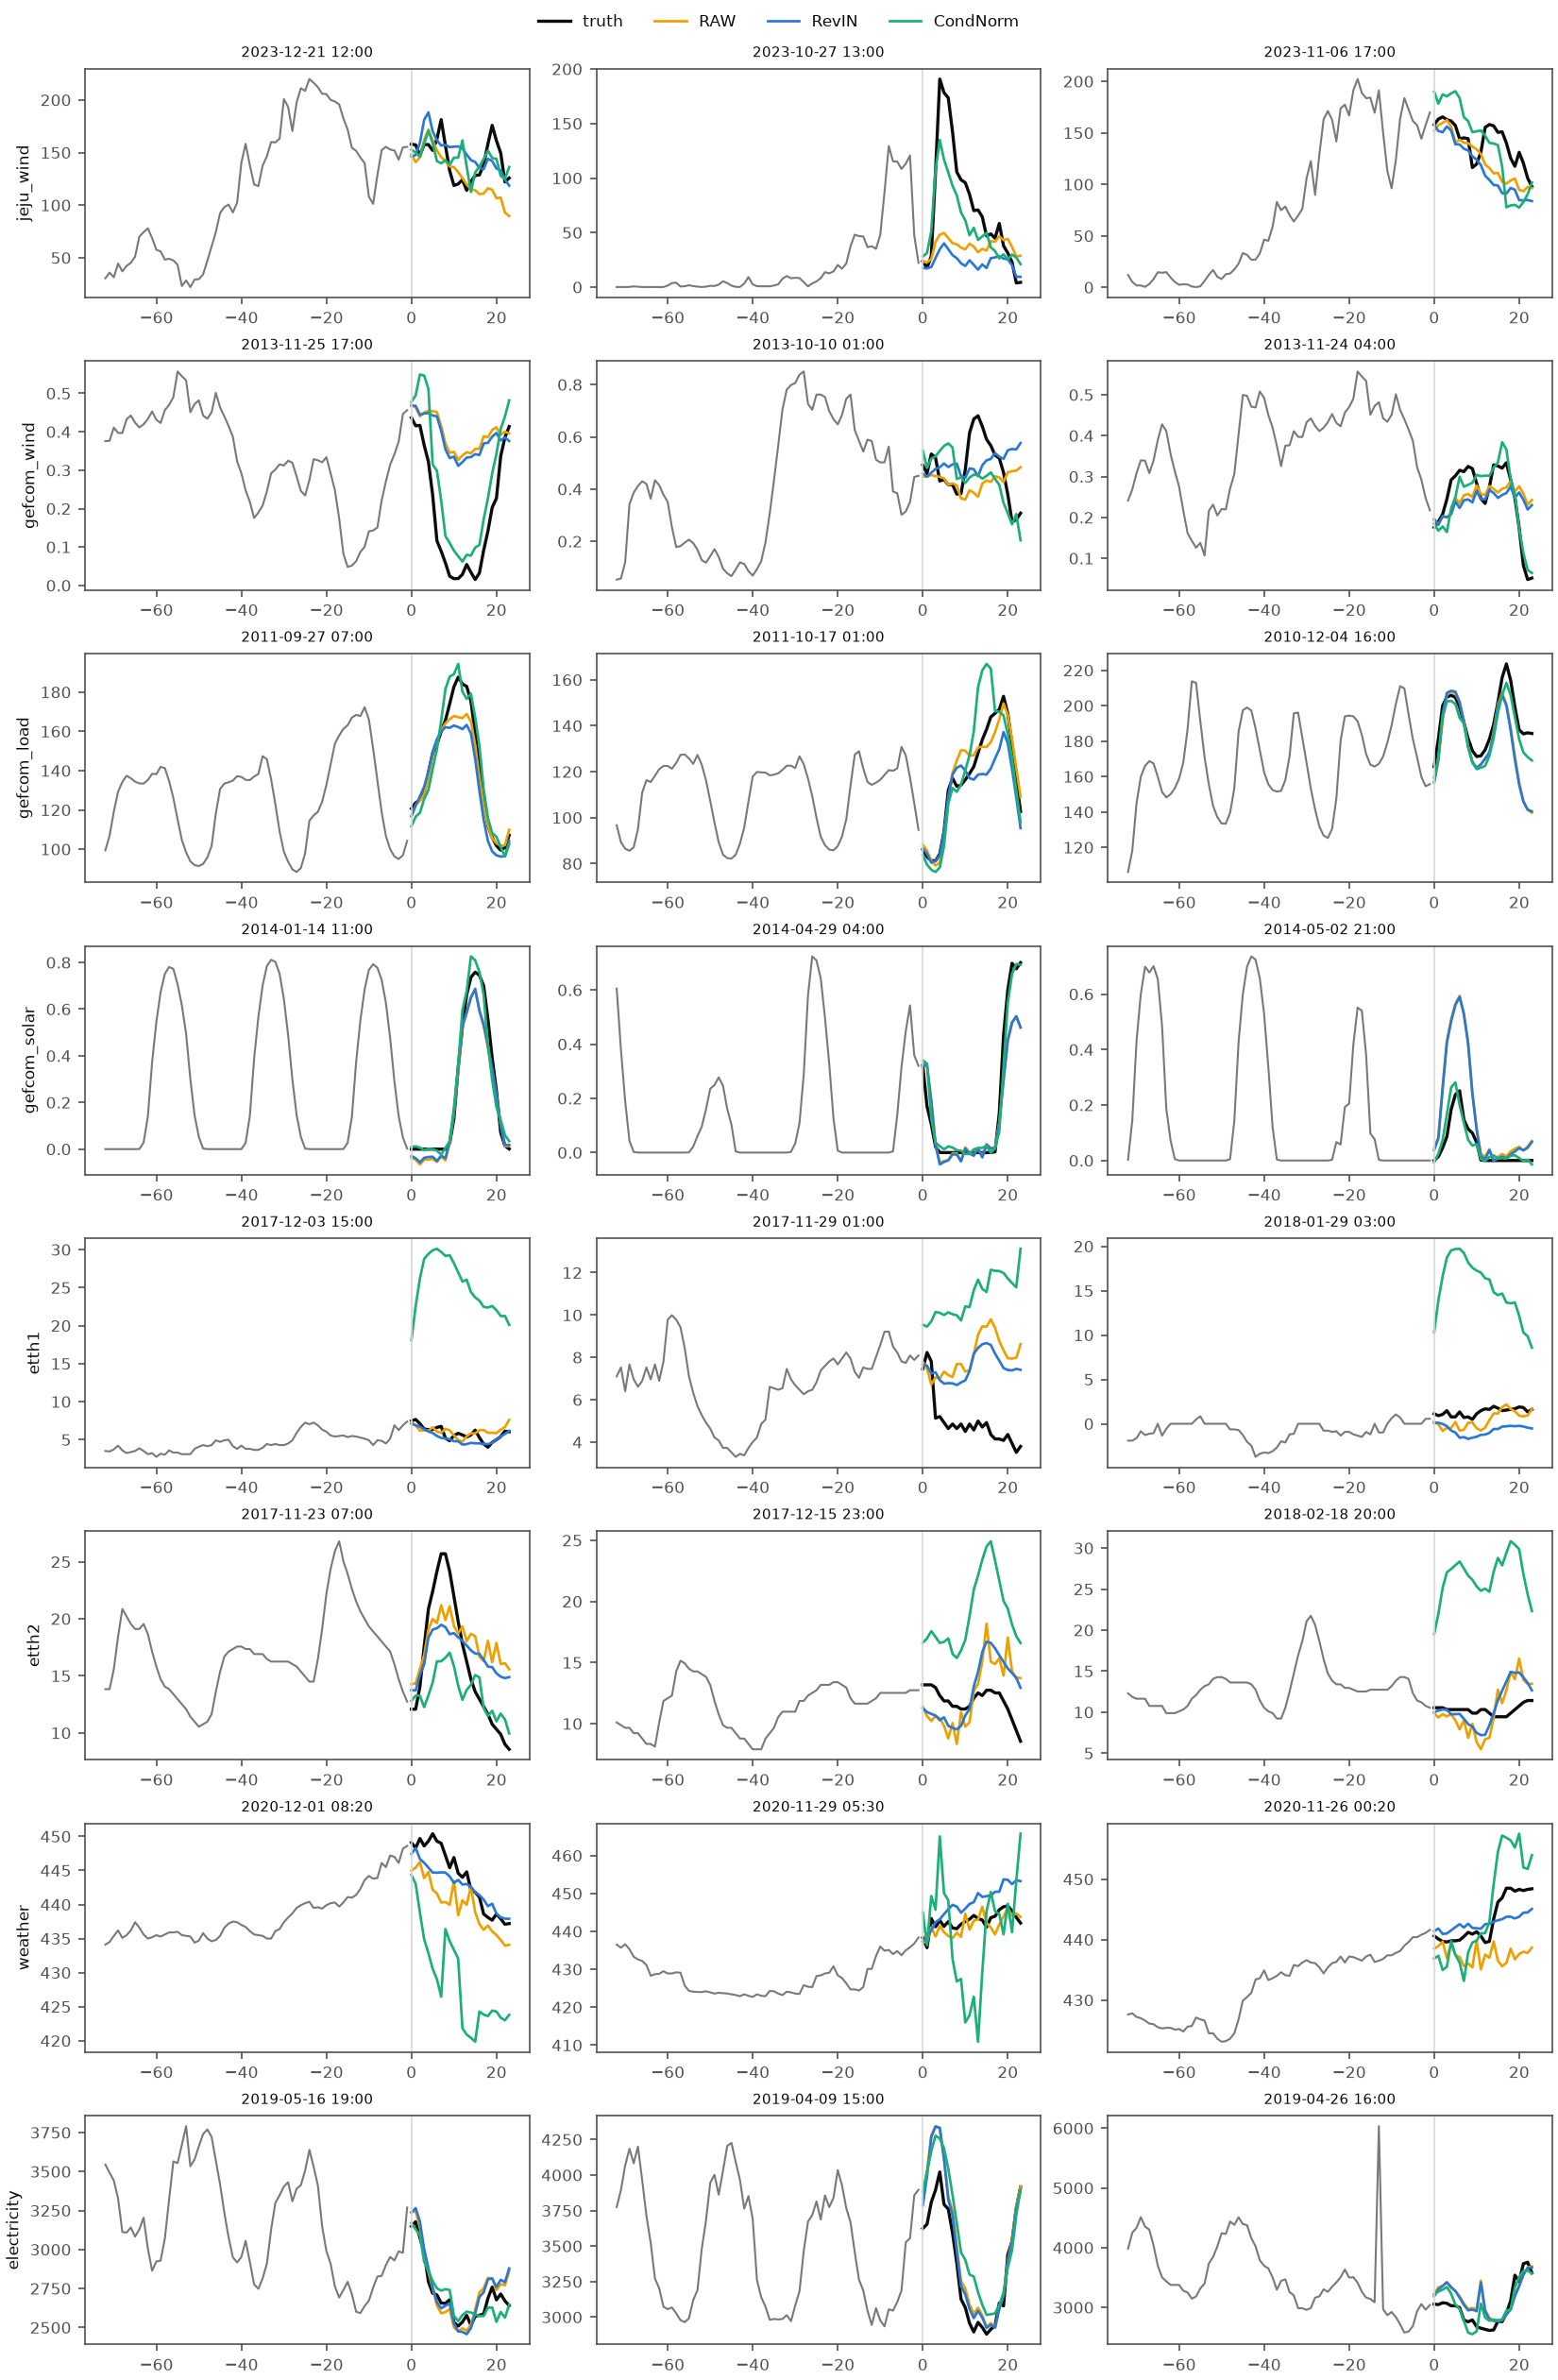
\includegraphics[keepaspectratio,width=\textwidth,height=0.8\textheight]{figures/sample_forecasts.png}
\caption{Qualitative test-set examples (identical backbone and information
set): one row per dataset, three sample windows per row; grey is the lookback,
black the ground truth, and colored lines the \rawm{}, RevIN, and CondNorm
forecasts. See the accompanying text for the reading of the wind, solar, and
standard-benchmark rows.}
\label{fig:samples}
\end{figure}

\section{Post-Hoc Hardening Evidence}\label{app:g7}

Everything in this appendix was produced \emph{after} the pre-registered
analysis was frozen, as part of an audit-and-hardening pass. None of it
alters any pre-registered number; all comparisons are internal to this
appendix (block self-containment, \Cref{app:design}).

\subsection{A nonlinear check of Proposition~1}\label{app:g7-mlp}

The structural half of \Cref{prop:deficiency}---that the composed forecast
\Cref{eq:equivariance} is additively separable in the window mean with unit
slope---holds for an arbitrary backbone and needs no check. What is specific
to linear classes is the \emph{quantification}, \Cref{eq:prop1,eq:prop1b}. To
probe whether that geometry survives nonlinearity, we train an identical
two-hidden-layer MLP ($128\times128$, ReLU) under the interaction DGP of
\Cref{sec:theory} in three arms that differ only in the normalization
constraint (\rawm{}, RevIN-style mean removal and restoration, \cnm{}-style
covariate restoration), at $\lambda \in \{0.4, 0.8\}$ with ten seeds, and
measure excess risk over the analytic Bayes predictor.
\Cref{fig:mlpdemo} shows the result: the RevIN-constrained arm cannot go
below the class floor $\kappa^2\,\var(\bar y \mid g)\,\var(g)$ (its mean
sits above the floor by at least $16$ standard errors of the mean at both
$\lambda$), while the unconstrained and covariate-restored arms sit roughly
a factor of twenty below it. That floor is \Cref{eq:prop1c} evaluated at
this configuration: the demo fixes $a = 1$, at which the pinned-slope term
vanishes identically and the whole irreducible excess is the interaction
term $\kappa^2 \var(g)\var(\bar y)(1-\varrho^2) = \kappa^2\var(g)\var(\bar
y \mid g)$. Earlier versions of this appendix carried the constant as
provisional and configurable pending a derivation; Step~7 of
\Cref{app:proofs} supplies it, so the demonstration now serves as a
nonlinear \emph{confirmation} of \Cref{eq:prop1c} rather than a measurement
against a guessed scale. It is also the cleanest illustration of the
proposition's division of labour: because $a=1$ here, nothing in this
figure is attributable to the pinned slope, and the entire gap between the
RevIN arm and the unconstrained arm is the interaction cost that only the
constrained class still pays.

\begin{figure}[htbp]
\centering
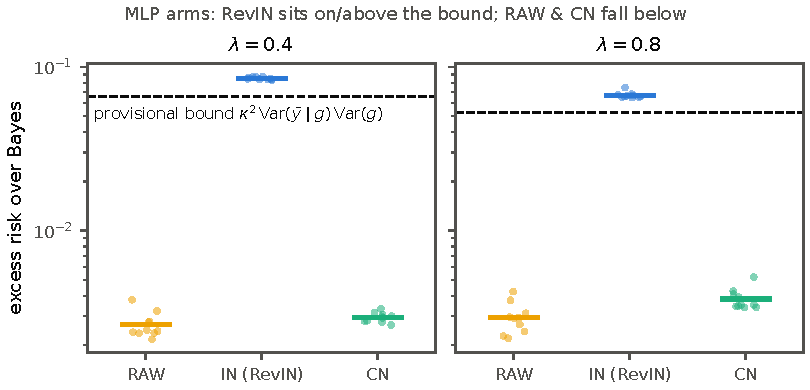
\includegraphics[width=.85\textwidth]{figures/figG_prop1_mlp.pdf}
\caption{Nonlinear check of Proposition~1. Excess risk over the Bayes
predictor for an identical MLP backbone under three normalization
constraints (ten seeds; dots are seeds, bars are means; dashed line is the
provisional RevIN-class floor $\kappa^2\,\var(\bar y \mid g)\,\var(g)$).
The RevIN-constrained arm is pinned above the floor at both $\lambda$;
the unconstrained (\rawm{}) and covariate-restored (\cnm{}) arms are not.}
\label{fig:mlpdemo}
\end{figure}

\subsection{Classical and diagnostic baselines (Block~E)}\label{app:g7-blocke}

\Cref{tab:baselines} adds five reference arms on all eight datasets:
seasonal naive, hour-of-day/day-of-week climatology, the CondNorm first
stage used \emph{alone} as a forecaster, a classical dynamic-regression
stand-in (ridge on lagged target plus target-time covariates, direct
multi-step), and the published-default \texttt{revin\_all} ablation with
its in-block comparators. Three observations. First, on the
exogenously-driven group the first stage alone is already competitive with
the full CondNorm pipeline (e.g., Jeju Wind $0.294$ vs.\ $0.307$;
GEFCom-Wind $0.156$ vs.\ $0.180$): most of conditional normalization's
value on these series is the covariate-to-level map itself, with the
backbone adding shape refinement --- and the same arm collapses on the
standard group (ETTh2 $3.37$), exactly as the boundary predicts. Second,
dynamic regression is competitive on wind ($0.285$ on Jeju) but loses
badly on the nonlinear temperature--load relation ($0.371$ vs.\ $0.108$),
supporting the nonlinear first stage. Third, \texttt{revin\_all}
(window-normalizing covariate channels as published defaults do) stays
within $\pm 0.05$ MSE of target-only normalization on seven of the eight
datasets --- significantly better on one (GEFCom-Wind), significantly
worse on two (Electricity, GEFCom-Load), within seed-level noise on the
remaining four --- but diverges catastrophically on GEFCom-Solar (MSE in
the hundreds at $h=336$, all seeds): an intermittent precipitation
covariate has window standard deviations down to $4\times10^{-6}$ ---
$1/800$ of its global scale --- so window normalization amplifies it
explosively. This is a reproducible
failure case for the published default and the reason our protocol
normalizes the target channel only (\Cref{app:design}).

\begin{table}[htbp]
\centering
\caption{Block~E baselines and ablation (post-hoc hardening block; not
pre-registered): test MSE (global z-score scale; dataset mean over horizons
and seeds). \emph{f/s only} = CondNorm first stage used alone;
\emph{dynreg} = ridge dynamic-regression stand-in; \emph{revin\_all} =
instance normalization applied to covariate channels as well (published
default), with its in-block linmix comparators. \textbf{Bold}: lowest MSE
per row. Self-contained block; no cross-block comparison.}
\label{tab:baselines}
\scriptsize
\setlength{\tabcolsep}{4pt}
\begin{tabular}{@{}lrrrrrrrr@{}}
\toprule
Dataset & s.naive & climat. & f/s only & dynreg & revin\_all & linmix\,\rawm & linmix\,RevIN & linmix\,\cnm \\
\midrule
Jeju Wind    & 1.627 & 1.032 & 0.294 & \textbf{0.285} & 0.349 & 0.344 & 0.367 & 0.307 \\
GEFCom-Wind  & 1.988 & 1.231 & \textbf{0.156} & 0.171 & 0.275 & 0.265 & 0.327 & 0.180 \\
GEFCom-Load  & 0.686 & 1.190 & 0.136 & 0.371 & 0.409 & 0.358 & 0.381 & \textbf{0.108} \\
GEFCom-Solar & 0.333 & 0.203 & \textbf{0.057} & 0.141 & 316.0 & 0.159 & 0.162 & 0.064 \\
ETTh1        & 0.670 & 0.883 & 1.403 & 0.479 & 0.396 & 0.397 & \textbf{0.391} & 2.993 \\
ETTh2        & 0.577 & 3.128 & 3.367 & 0.892 & 0.272 & 0.361 & \textbf{0.270} & 7.392 \\
Weather      & 0.338 & 0.688 & 0.648 & \textbf{0.181} & 0.183 & 0.185 & 0.182 & 1.069 \\
Electricity  & 0.217 & 0.389 & 0.322 & 0.199 & 0.199 & 0.205 & \textbf{0.148} & 0.175 \\
\bottomrule
\end{tabular}
\end{table}

\subsection{Probabilistic robustness (Block~F)}\label{app:g7-blockf}

We re-ran the boundary comparison with quantile forecasting: an RLinear
backbone with a nine-quantile pinball head (Block-A capacities and
lookbacks; all five arms, per-quantile denormalization, non-crossing by
sorting) and a LightGBM quantile backbone (levels $\{0.1,0.5,0.9\}$; arms
as in Block~A). \Cref{tab:prob} reports mean pinball loss and empirical
80\% coverage. The boundary persists in full: CondNorm attains the lowest
pinball in $11/11$ exogenous (dataset,\,$h$) cells on \emph{both}
backbones (mean pinball $0.106$ vs.\ RevIN's $0.197$ on the linear
backbone, a $46\%$ improvement), and the ordering reverses on the standard
group exactly as in Block~A. The relative gap is smaller than under
squared error, as expected when moving from a squared to a
$1$-homogeneous loss. Calibration is the one metric where CondNorm does
not dominate: its 80\% intervals cover $0.60$ on the exogenous group
against RevIN's $0.82$ (nominal $0.80$), with the miscoverage split
roughly evenly between the two tails ($P(y \le q_{0.1}) = 0.19$ vs.\
nominal $0.10$; $P(y > q_{0.9}) = 0.21$ vs.\ nominal $0.10$) --- the
intervals are under-dispersed on both sides. Sharp but symmetrically
under-covered intervals are the probabilistic signature of an unpropagated
variance term ($\sest$ in \Cref{sec:theory}); propagating first-stage
uncertainty into the quantile spread is a natural extension we leave to
future work.

\begin{table}[htbp]
\centering
\caption{Block~F probabilistic robustness (post-hoc hardening block; not
pre-registered): mean pinball loss (empirical 80\% coverage in
parentheses; nominal $0.80$), dataset mean over horizons and seeds. \textbf{Bold}: lowest pinball per row within the backbone.
LightGBM SAN/FAN are structurally N/A as in Block~A; \emph{winz} is the
window z-normalization arm. CRPS approximations preserve the pinball
ordering and are omitted.}
\label{tab:prob}
\scriptsize
\setlength{\tabcolsep}{2.2pt}
\begin{tabular}{@{}lccccc|ccc@{}}
\toprule
 & \multicolumn{5}{c|}{RLinear-Q (9 quantiles)} & \multicolumn{3}{c}{LightGBM-Q ($\{0.1,0.5,0.9\}$)} \\
Dataset & \rawm & RevIN & SAN & FAN & \cnm & \rawm & winz & \cnm \\
\midrule
Jeju Wind    & .223 (.79) & .228 (.80) & .237 (.73) & .284 (.39) & \textbf{.165} (.58) & .182 (.68) & .186 (.71) & \textbf{.134} (.64) \\
GEFCom-Wind  & .320 (.76) & .313 (.79) & .320 (.57) & .431 (.19) & \textbf{.135} (.50) & .257 (.68) & .244 (.71) & \textbf{.105} (.60) \\
GEFCom-Load  & .162 (.83) & .165 (.80) & .167 (.78) & .173 (.75) & \textbf{.085} (.66) & .136 (.74) & .132 (.75) & \textbf{.073} (.65) \\
GEFCom-Solar & .092 (.89) & .092 (.89) & .101 (.84) & .108 (.78) & \textbf{.058} (.65) & .062 (.84) & .066 (.79) & \textbf{.044} (.71) \\
\midrule
ETTh1        & .163 (.79) & \textbf{.160} (.82) & .166 (.73) & .178 (.66) & .604 (.14) & .125 (.77) & \textbf{.122} (.73) & .354 (.38) \\
ETTh2        & .146 (.78) & \textbf{.136} (.74) & .139 (.68) & .155 (.66) & 1.126 (.03) & .168 (.70) & \textbf{.112} (.71) & .616 (.17) \\
Weather      & .096 (.87) & \textbf{.087} (.73) & .089 (.70) & .094 (.86) & .245 (.45) & .070 (.85) & \textbf{.067} (.76) & .200 (.49) \\
Electricity  & .102 (.83) & \textbf{.100} (.82) & .102 (.78) & .101 (.81) & .110 (.65) & .077 (.80) & \textbf{.076} (.79) & .092 (.71) \\
\bottomrule
\end{tabular}
\end{table}

\subsection{Supporting inference for the LPS values}\label{app:g7-lpsinf}

\Cref{tab:lpsinf} adds three post-hoc inferential quantities to the
pre-registered LPS values, all computed under the identical LPS protocol:
a permutation $p$-value against stride-preserving circular shifts of the
covariates (with a season-aligned variant restricting shifts to whole
weeks), a moving-block bootstrap 90\% interval, and a rough plug-in
estimate $\hat{\lambda}^{*}$ of the crossover from measurable quantities.
The exogenous group is uniformly significant ($p \le .008$) with intervals
above $\tau$; the standard group is uniformly compatible with the null.
The plug-in $\hat{\lambda}^{*}$ ordering agrees with the realized winner
on all eight datasets (negative values --- CN dominant at every $\lambda$
--- for the wind datasets; values above one --- IN dominant --- for the
standard group). Electricity is the boundary case on every diagnostic at
once ($\lps=.283$, $p=.058$, $\hat{\lambda}^{*}=1.35$, realized gap
$-0.027$), consistent with its pre-registered lowest-confidence flag.
Bootstrap intervals for negative-LPS series are biased upward (block
resampling dilutes the across-fold drift that produces negative
out-of-sample $R^2$), so the permutation $p$-value is the informative
quantity there.

\begin{table}[htbp]
\centering
\caption{Post-hoc inference for the pre-registered LPS values (identical
protocol: $w=96$, LightGBM first stage, expanding chronological CV).
$p_{\mathrm{perm}}$: circular-shift permutation ($B \le 999$, exact where
enumerable); aligned: shifts restricted to whole weeks; CI: moving-block
bootstrap, 90\%; $\hat{\lambda}^{*}$: plug-in crossover estimate at
$h=96$ (negative $\Rightarrow$ CN dominates all $\lambda$;
$>1 \Rightarrow$ IN dominates). The decision rule remains the
pre-registered $\lps \ge \tau$.}
\label{tab:lpsinf}
\small
\begin{tabular}{@{}lrrrrr@{}}
\toprule
Dataset & $\lps$ & $p_{\mathrm{perm}}$ & aligned & 90\% CI & $\hat{\lambda}^{*}$ \\
\midrule
Jeju Wind    & $.745$  & $.006$ & $.039$ & $[.76,\,.88]$ & $-0.20$ \\
GEFCom-Wind  & $.744$  & $.008$ & $.059$ & $[.70,\,.85]$ & $-0.51$ \\
GEFCom-Load  & $.894$  & $.002$ & $.011$ & $[.90,\,.95]$ & $0.68$ \\
GEFCom-Solar & $.875$  & $.005$ & $.035$ & $[.88,\,.95]$ & $0.09$ \\
ETTh1        & $-.717$ & $.39$  & $.38$  & $[-.02,\,.40]$ & $2.26$ \\
ETTh2        & $-.205$ & $.19$  & $.19$  & $[-.29,\,.42]$ & $2.90$ \\
Weather      & $.110$  & $.36$  & $.41$  & $[-.22,\,.66]$ & $1.02$ \\
Electricity  & $.283$  & $.058$ & $.075$ & $[.38,\,.57]$ & $1.35$ \\
\bottomrule
\end{tabular}
\end{table}


\clearpage  % flush appendix floats before the bibliography
\bibliographystyle{elsarticle-harv}
\bibliography{references}

\end{document}
